\documentclass[11pt,a4paper]{article}

% ---------------------------------------------------------------- packages
\usepackage[T1]{fontenc}
\usepackage[utf8]{inputenc}
\usepackage{lmodern}
\usepackage{microtype}
\usepackage[a4paper,margin=2.3cm]{geometry}
\usepackage{graphicx}
\usepackage{booktabs}
\usepackage{tabularx}
\usepackage{array}
\usepackage{multirow}
\usepackage{float}
\usepackage[font=small,labelfont=bf]{caption}
\usepackage{enumitem}
\usepackage{amsmath}
\usepackage{xcolor}
\usepackage{tikz}
\usetikzlibrary{arrows.meta,positioning}
\usepackage[numbers,sort&compress]{natbib}
\usepackage[hidelinks]{hyperref}

\setlist{itemsep=1pt,topsep=3pt}
\newcolumntype{L}{>{\raggedright\arraybackslash}X}
\renewcommand{\arraystretch}{1.12}
\setlength{\parskip}{4pt}
\setlength{\parindent}{0pt}
\setlength{\emergencystretch}{3em}
\graphicspath{{figures/}}

\newcommand{\code}[1]{\texttt{#1}}

% ---------------------------------------------------------------- title
\title{\textbf{Edge-Ready ECG Heartbeat Classification using CRISP-DM}\\[6pt]
\large Final report: CRISP-DM stages 1--6\\[4pt]
\normalsize D7043E Advanced Data Mining, Lule\aa{} University of Technology}
\author{Group 15\\[6pt]
\begin{tabular}{l l}
Achyuth Kumar Baddela & \href{mailto:achbad-5@student.ltu.se}{achbad-5@student.ltu.se}\\
Sathish Kumaresan & \href{mailto:satkum-5@student.ltu.se}{satkum-5@student.ltu.se}\\
Suresh Balaraman & \href{mailto:surbal-4@student.ltu.se}{surbal-4@student.ltu.se}
\end{tabular}}
\date{November 2026}

\begin{document}
\maketitle

\begin{abstract}
\noindent
We classify single heartbeats from an ECG into four classes (N, S, V and F) with a small model made for the Analog Devices MAX78002 microcontroller, following the six CRISP-DM stages~\citep{chapman2000crisp,wirth2000crisp}. Task 1 (Sections 1--3) defines the problem and measurable success criteria, analyses the MIT-BIH data and prepares 100,607 beats from 44 records, split by patient; a test on the training data shows why the split matters (macro F1 0.875 with a random beat split against 0.492 with patients held out). Task 2 (Sections 4--9) trains a random-forest baseline and a 1D CNN with 10,004 parameters, compares FP32, INT16 and INT8 versions, and evaluates once on 22 unseen patients: macro F1 0.611 in FP32 and 0.664 for the INT8 model trained with quantisation-aware training, against 0.475 for the baseline. Under real noise the model degrades gradually except for electrode motion. The INT8 model passes the Analog Devices toolchain and is synthesised to C code using 0.4\,\% of the chip's weight memory. All numbers come from the submitted code. This is a student project, not a medical device.
\end{abstract}

{\small\tableofcontents}
\newpage

% =====================================================================
\part*{Task 1: Business Understanding, Data Understanding and Data Preparation}
\addcontentsline{toc}{part}{Task 1: Business Understanding, Data Understanding and Data Preparation}

\section{Business/Application Understanding}
% =====================================================================

\subsection{Application Scenario}

\textbf{Problem.} Many heart rhythm problems, such as extra beats from the atria or ventricles, come and go. A short ECG at the clinic often misses them, so patients wear a Holter monitor or a patch for days or weeks. That produces about 100,000 beats per day, which is far too many for a person to check one by one. We want a model that labels every beat as normal-type (N), supraventricular ectopic (S), ventricular ectopic (V) or fusion (F).

\textbf{Where it is useful.} Pre-screening long Holter and patch recordings, flagging unusual beats for a technician, counting how often they occur (for example V beats per hour), and remote monitoring of patients after surgery or at high risk.

\textbf{Why run it on the device.} If the wearable classifies beats itself, it only needs to send a few events instead of the full 360~Hz signal. This saves battery, because the radio uses most of the power. It also keeps raw ECG private, works without a phone connection, and makes long-term monitoring cheaper.

\textbf{Users.} Device makers, Holter technicians, clinicians who receive summaries, and researchers. A clinician always makes the final diagnosis.

\subsection{Data-Mining Objective}

\begin{description}[leftmargin=2.2cm,style=nextline]
  \item[Input] One array of size $2 \times 256$ per annotated heartbeat.
  Channel~0 is a 2-second window of the MLII lead (1.25~s before and 0.75~s after the beat). It is filtered to 0.5--40~Hz, resampled from 360~Hz to 128~Hz, scaled per patient and clipped to $[-1, 127/128]$, the 8-bit input range of the MAX78002.
  Channel~1 holds the RR ratio of the beat minus one (time since the previous beat divided by the average of the 10 intervals before it).
  \item[Output] One of the four AAMI classes~\citep{aami2012ec57}: N, S, V or F. The model gives four scores and we take the highest.
  \item[Type of task] Supervised multiclass classification (4 classes) with strong class imbalance, trained and tested on different patients.
\end{description}

\subsection{Project Objectives}
\begin{enumerate}
  \item Tell N, S, V and F beats apart, using the standard MIT-BIH labels.
  \item Work on new patients: train and tune only on DS1 records and test once on DS2.
  \item Find the rare classes (S, V, F) even though 90\,\% of beats are N.
  \item Stay reliable with realistic noise at 12, 6 and 0~dB.
  \item Build a small 1D CNN that uses only operations the MAX78002 supports.
  \item Quantise the model and compare FP32, INT16 and INT8 on size and accuracy.
  \item Prepare it with the Analog Devices tools (ai8x-training and ai8x-synthesis~\citep{adi_ai8x_training,adi_ai8x_synthesis}) and judge whether it fits the device.
\end{enumerate}

\subsection{Success Criteria}

All criteria are measured once on DS2, after the final model is chosen. Every earlier decision uses DS1 only. For comparison, a model that always answers ``N'' gets about 90\,\% accuracy but only about 0.24 macro F1. Results on new patients are known to be much lower than results with random splits~\citep{dechazal2004automatic,luz2016survey,llamedo2011heartbeat}, so the targets for the rare classes are modest.

\begin{table}[H]
\centering
\small
\caption{Success criteria (measured on DS2 unless stated otherwise).}
\label{tab:success}
\begin{tabularx}{\textwidth}{@{} l l L c c @{}}
\toprule
Area & ID & Criterion & Target & Stretch \\
\midrule
\multirow{3}{*}{Predictive performance}
 & P1 & Macro F1 (N, S, V, F), FP32 model, clean DS2 & $\geq 0.60$ & $\geq 0.70$ \\
 & P2 & Macro F1 gain over the simple baseline & $\geq +0.05$ & $\geq +0.10$ \\
 & P3 & N recall (keeps false alarms low) & $\geq 0.90$ & $\geq 0.95$ \\
\midrule
\multirow{3}{*}{Minority classes}
 & M1 & V recall / V precision & $\geq 0.80$ / $\geq 0.70$ & $\geq 0.90$ / $\geq 0.85$ \\
 & M2 & S recall / S precision & $\geq 0.60$ / $\geq 0.40$ & $\geq 0.75$ / $\geq 0.55$ \\
 & M3 & F recall & $\geq 0.25$ & $\geq 0.40$ \\
\midrule
\multirow{3}{*}{Noise robustness}
 & R1 & Drop in macro F1 at 12~dB (mean over bw, ma, em) & $\leq 0.05$ & $\leq 0.02$ \\
 & R2 & Drop in macro F1 at 6~dB (mean over bw, ma, em) & $\leq 0.10$ & $\leq 0.05$ \\
 & R3 & V recall at 0~dB (mean over bw, ma, em) & $\geq 0.50$ & $\geq 0.70$ \\
\midrule
\multirow{3}{*}{Model complexity}
 & C1 & Trainable parameters & $\leq 100{,}000$ & $\leq 50{,}000$ \\
 & C2 & INT8 weight memory (course design target: 2~MB) & $\leq 100$~KB & $\leq 50$~KB \\
 & C3 & Multiply--accumulate operations per beat & $\leq 5$~M & $\leq 2$~M \\
\midrule
\multirow{3}{*}{Quantisation}
 & Q1 & FP32, INT16 and INT8 compared on size, accuracy and F1 & done & done \\
 & Q2 & INT8 macro F1 minus FP32 macro F1 & $\geq -0.02$ & $\geq -0.01$ \\
 & Q3 & INT16 macro F1 minus FP32 macro F1 & $\geq -0.005$ & $\geq -0.002$ \\
\midrule
\multirow{2}{*}{MAX78002 compatibility}
 & H1 & Only supported layers (Conv1d kernel 1--9, pooling, ReLU, small Linear) and a fixed $2 \times 256$ input & yes & yes \\
 & H2 & Toolchain: model accepted, quantised, synthesised, C files generated & 4 $\times$ PASS & 4 $\times$ PASS \\
\bottomrule
\end{tabularx}
\end{table}

We always report accuracy, but it is not a criterion because the N class dominates it. INT16 is a software comparison only, because the MAX78002 supports 1-, 2-, 4- and 8-bit weights, not 16-bit~\citep{adi_ai8x_training}.

\subsection{Constraints}

\begin{itemize}
  \item \textbf{Limited memory.} The MAX78002 stores up to 2 million 8-bit weights (2,340~KiB) and has 1,280~KiB of data memory~\citep{adi_max78002_datasheet,adi_ai8x_training}. The course treats 2~MB as a design target, not a hard limit. A small CNN uses a few percent of this, so the layer rules below matter more.
  \item \textbf{8-bit computation and supported layers.} Inputs, weights and activations are 8-bit integers. Conv1d kernels must be 1--9 samples long with stride 1, pooling is 1--16, activations are ReLU or none, and a fully connected layer has at most 1,024 inputs and outputs~\citep{adi_ai8x_training}. Recurrent layers and attention are not available.
  \item \textbf{Class imbalance.} About 90\,\% of beats are N and less than 1\,\% are F.
  \item \textbf{Few patients.} We use 44 records from 43 people. Rare classes come from very few of them: 95\,\% of the training F beats are from record 208.
  \item \textbf{Noise.} Wearable ECG is noisier than these clinical recordings. We must test with real noise without leaking it into training.
  \item \textbf{Computing.} Preprocessing takes about one minute on a normal CPU. Training will run on a laptop CPU or Google Colab. The ai8x tools need Linux and their own Python setup.
  \item \textbf{No hardware.} We have no MAX78002 board, so we will not claim measured speed, power or on-device accuracy.
\end{itemize}

\textbf{Tools.} We use Python for every stage (wfdb, NumPy, SciPy, pandas, scikit-learn, Matplotlib, PyTorch in Task 2). RapidMiner is allowed, but quantisation and the ai8x tools need Python anyway, so one Python code base keeps everything reproducible.

\subsection{Risks and Challenges}

\begin{table}[H]
\centering
\small
\caption{Main risks and how we handle them.}
\label{tab:risks}
\begin{tabularx}{\textwidth}{@{} >{\raggedright\arraybackslash}p{3.0cm} L L @{}}
\toprule
Risk & Why is it important? & Proposed mitigation \\
\midrule
Data leakage & Beats from one patient look almost the same. A random split raised macro F1 from 0.49 to 0.88 in our test (Section~\ref{sec:leakage}). & Split by record only; keep DS2 untouched until the end; the code checks that the splits do not overlap. \\
Class imbalance & An ``always N'' model scores 90\,\% accuracy. Training F beats come almost only from one patient. & Class weights, macro F1 for model choice, per-class results, augmentation. \\
Differences between patients & Beat height differs 4.4 times between records, and beat shapes differ a lot. S beats often look normal and only arrive early. & Scale each record separately, add the RR channel, use a 2~s window that includes the previous beat. \\
Small validation set & Validation has only 21 F beats, so its scores are noisy. & Choose models by macro F1 plus S and V recall; report validation and test results side by side (Tables~\ref{tab:selection} and \ref{tab:clean}). \\
Loss after INT8 / toolchain failure & A model that loses accuracy after quantisation or cannot be synthesised misses the main goal. & Quantisation-aware training; use only ai8x layers; test synthesis early. \\
Noise & Electrode-motion noise can look like ectopic beats. & Test at 12/6/0~dB with real noise; add synthetic noise during training. \\
\bottomrule
\end{tabularx}
\end{table}

% =====================================================================
\section{Data Understanding}
% =====================================================================

\subsection{Dataset Description}

\begin{table}[H]
\centering
\small
\caption{MIT-BIH Arrhythmia Database~\citep{moody2001impact,goldberger2000physionet,physionet_mitdb}. Values marked $^{*}$ were checked in the downloaded files (\code{results/dataset\_summary.json}).}
\label{tab:dataset}
\begin{tabularx}{\textwidth}{@{} l L @{}}
\toprule
Property & Value \\
\midrule
Database & MIT-BIH Arrhythmia Database v1.0.0 (PhysioNet \code{mitdb}), recorded 1975--1979 \\
Records & 48$^{*}$ half-hour Holter recordings \\
Subjects & 47 (25 men aged 32--89, 22 women aged 23--89); records 201 and 202 are the same man \\
Channels and leads & 2 per record$^{*}$. Channel~0 is MLII in 45 records$^{*}$; record 114 has MLII in channel~1$^{*}$; paced records 102 and 104 have no MLII$^{*}$. Other leads: V1, V2, V4 or V5$^{*}$ \\
Sampling frequency & 360~Hz$^{*}$, 11-bit resolution$^{*}$ \\
Duration & 30.09~min per record$^{*}$ (650,000 samples), 24.07~h in total$^{*}$ \\
Annotations & One label per beat, checked by two cardiologists, plus rhythm and signal-quality notes. 112,647 annotations$^{*}$, of which 109,494 are beats$^{*}$ \\
Noise data & MIT-BIH Noise Stress Test Database~\citep{moody1984noise,physionet_nstdb}: 30~min of baseline wander (\code{bw}), muscle noise (\code{ma}) and electrode motion (\code{em}) \\
\bottomrule
\end{tabularx}
\end{table}

\subsection{Target Classes}

\begin{table}[H]
\centering
\small
\caption{Final classes, the MIT-BIH labels they contain, and beats after preparation (\code{results/symbol\_counts.csv}).}
\label{tab:classes}
\begin{tabularx}{\textwidth}{@{} l L r r r @{}}
\toprule
Class & Original annotations included (beats) & DS1 & DS2 & Total \\
\midrule
N & N normal (74,458), L left bundle branch block (8,068), R right bundle branch block (7,249), e atrial escape (16), j nodal escape (229) & 45,812 & 44,208 & 90,020 \\
S & A atrial premature (2,545), a aberrated atrial premature (150), J nodal premature (83), S supraventricular premature (2) & 943 & 1,837 & 2,780 \\
V & V premature ventricular contraction (6,899), E ventricular escape (106) & 3,786 & 3,219 & 7,005 \\
F & F fusion of ventricular and normal (802) & 414 & 388 & 802 \\
\midrule
Total & & 50,955 & 49,652 & 100,607 \\
\bottomrule
\end{tabularx}
\end{table}

\textbf{What we excluded and why} (\code{results/exclusions.csv}):
\begin{itemize}
  \item \textbf{Paced records} 102, 104, 107 and 217: their beats come from a pacemaker, which is outside the four-class task (AAMI recommendation).
  \item \textbf{Unclassifiable beats} (\code{Q}): 8 in DS1 and 7 in DS2, too few to learn and not one of the four classes.
  \item \textbf{Beats at the very start or end of a record} (110): their 2~s window would run past the signal. One more beat is dropped because it is the first in its record and has no RR interval.
  \item \textbf{Non-beat annotations}, such as rhythm changes (\code{+}), signal-quality notes (\code{\textasciitilde}), artefacts (\code{|}) and flutter waves (\code{!}), are not heartbeats. We still use the quality notes to find noisy parts.
\end{itemize}
In total 126 beats (0.13\,\%) of the 44 records are dropped.

\subsection{Exploratory Data Analysis}
\label{sec:eda}

All figures are made by \code{notebooks/EDA.ipynb}. We describe all records, but every decision uses DS1 only.

\textbf{Example ECG signal.} Figure~\ref{fig:example} shows 10~seconds of record 208. V beats are wide and flip direction in lead V1, the F beat looks in-between, and the two S beats look normal but come early.

\begin{figure}[H]
\centering
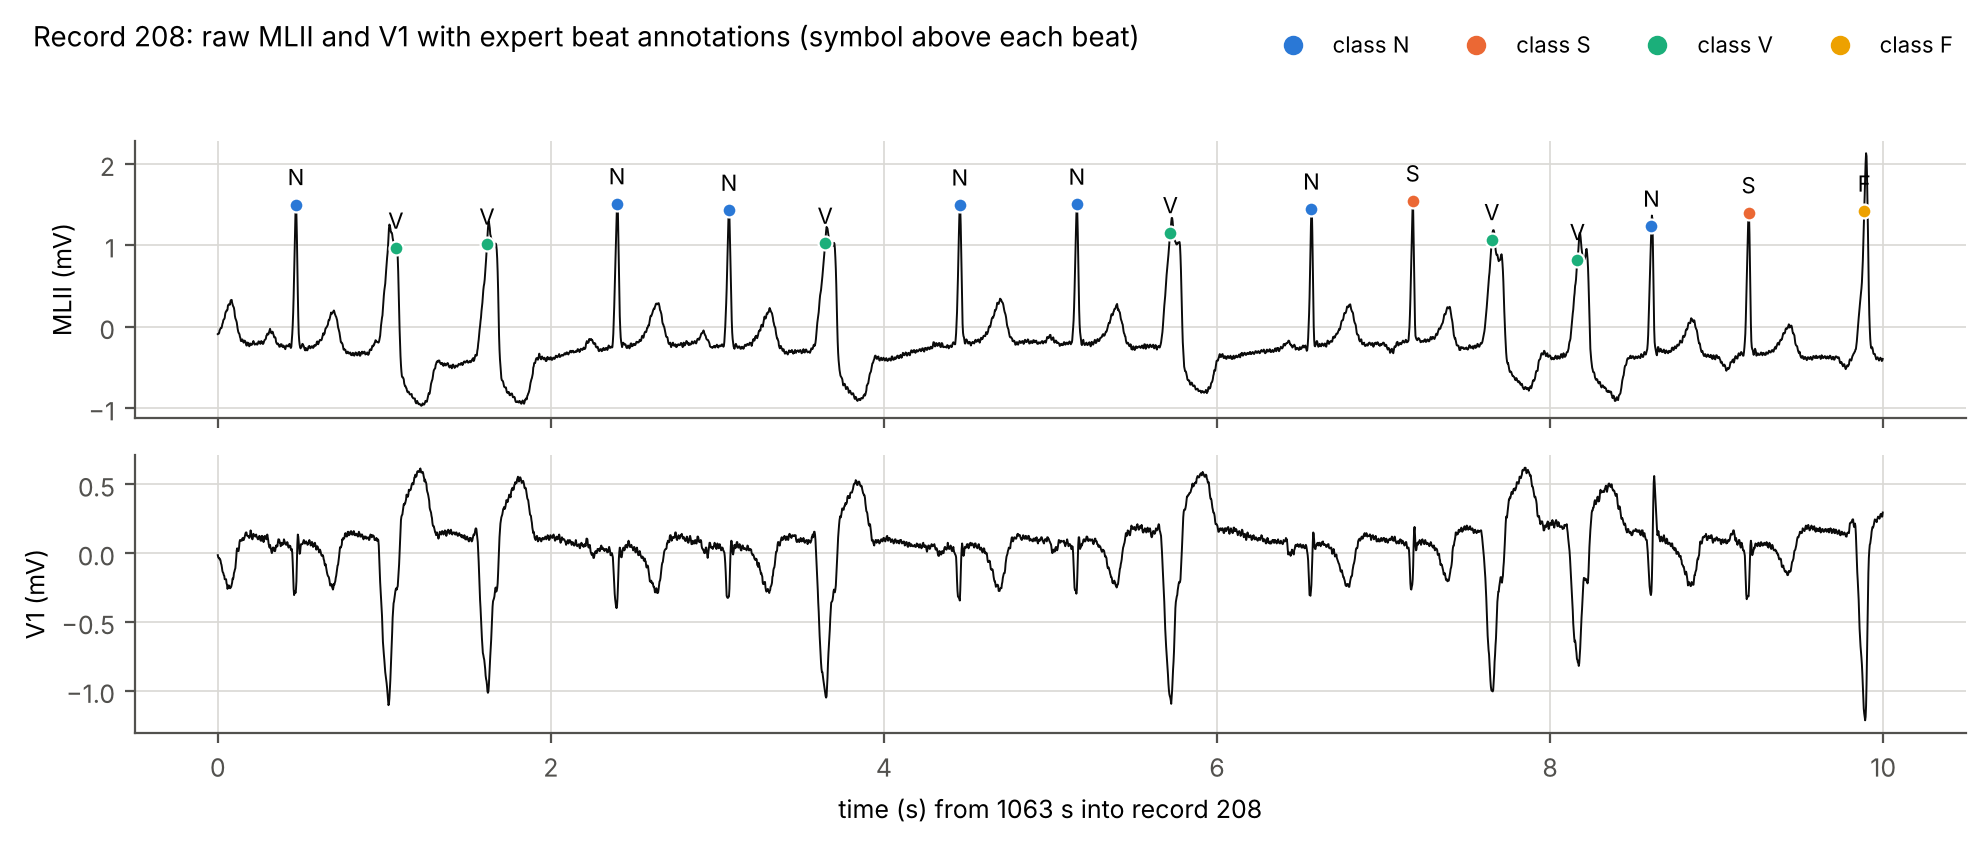
\includegraphics[width=\textwidth]{fig_example_ecg.png}
\caption{Record 208 with the experts' beat labels; dot colour shows the class.}
\label{fig:example}
\end{figure}

\textbf{Example beat from each class.} In Figure~\ref{fig:classbeats} the average S beat looks almost the same as the average N beat, so shape alone cannot separate them. Figure~\ref{fig:rr} shows what does: S and V beats come early (median RR ratio 0.80 and 0.72, against 1.00 for N and 0.95 for F). This is why the model gets a timing channel.

\begin{figure}[H]
\centering
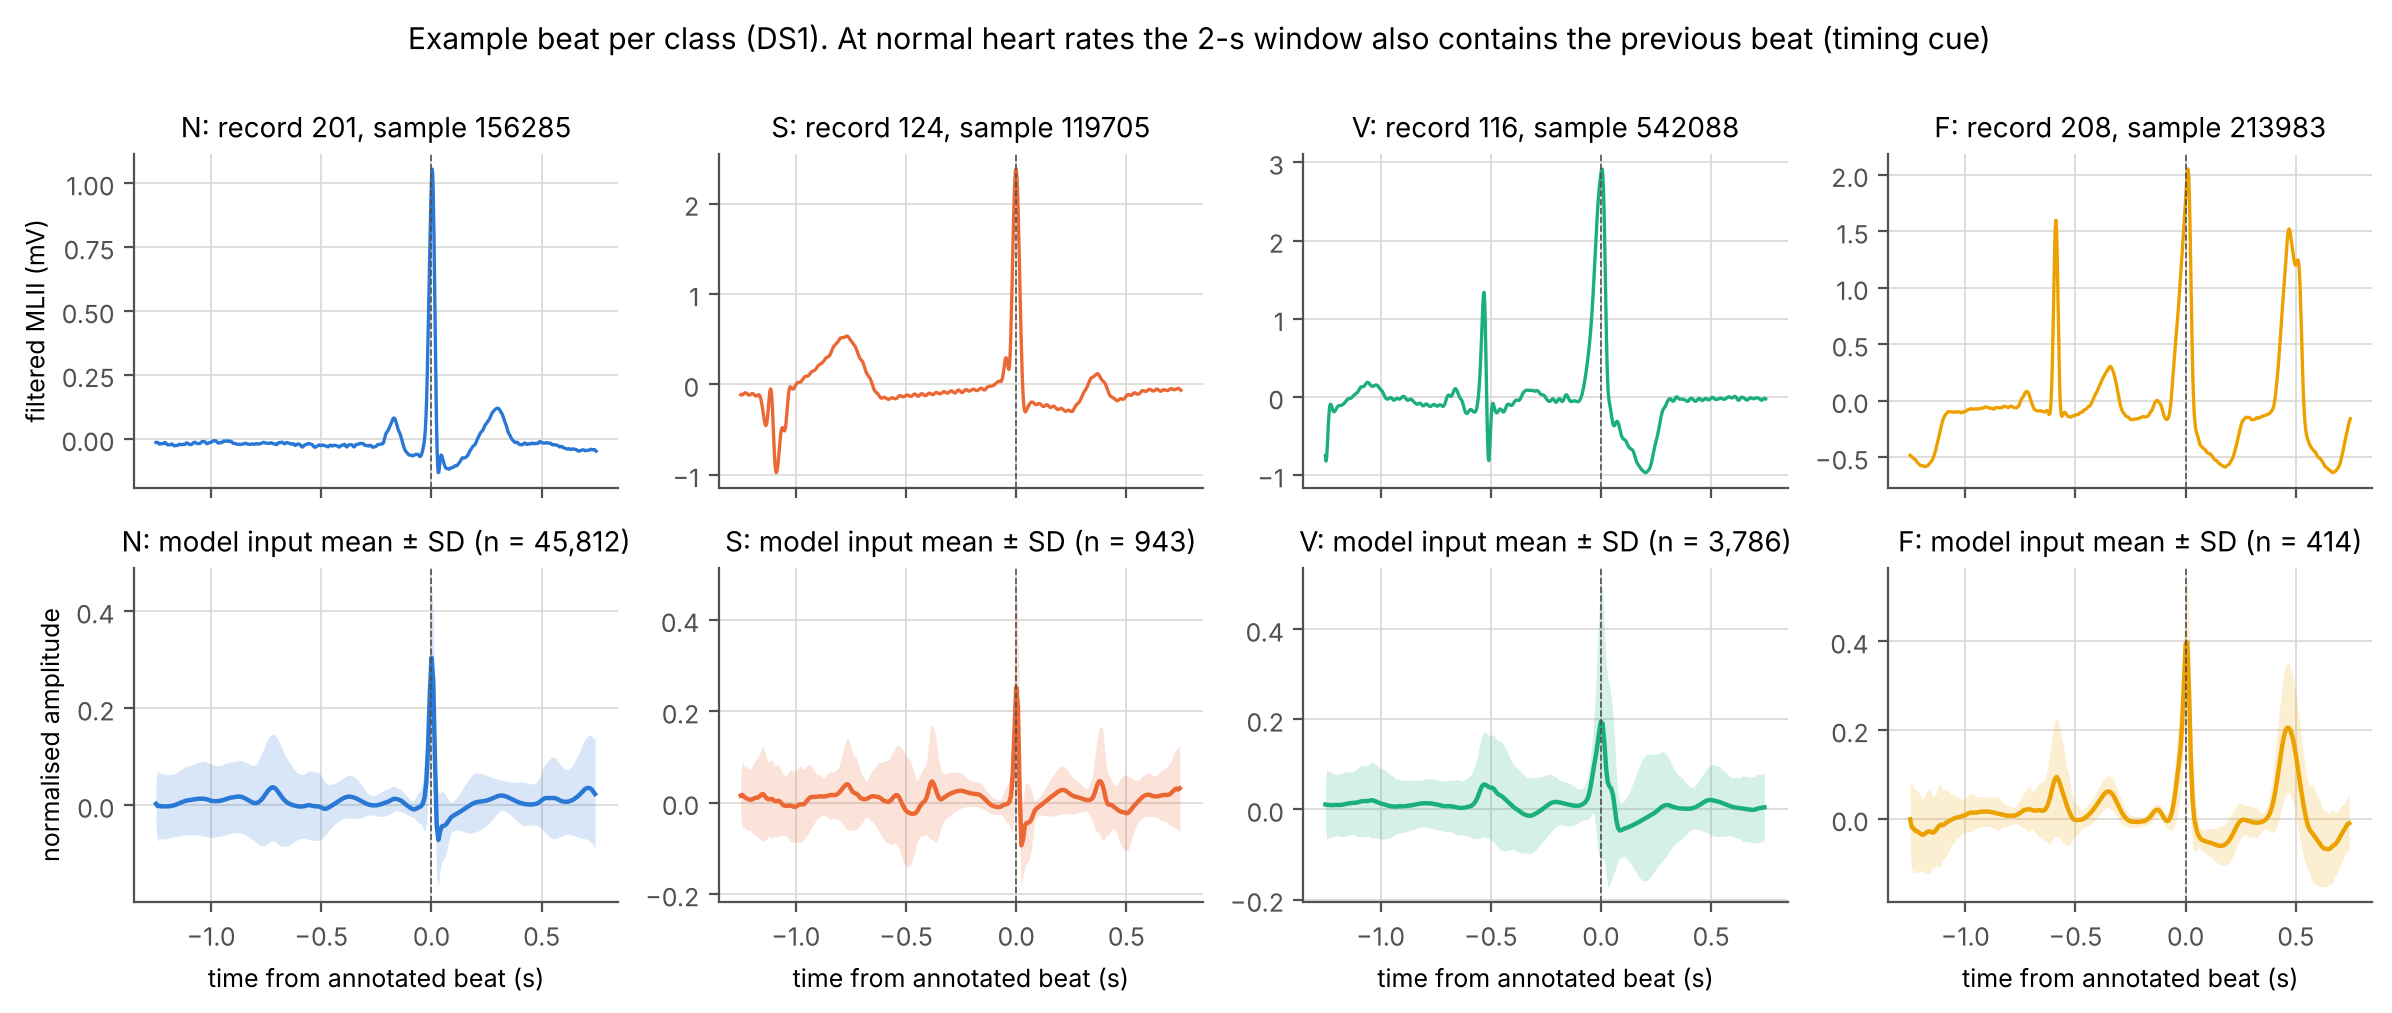
\includegraphics[width=\textwidth]{fig_class_beats.png}
\caption{Top: a typical beat of each class (mV). Bottom: model input, class average $\pm$ 1 standard deviation (DS1).}
\label{fig:classbeats}
\end{figure}

\begin{figure}[H]
\centering
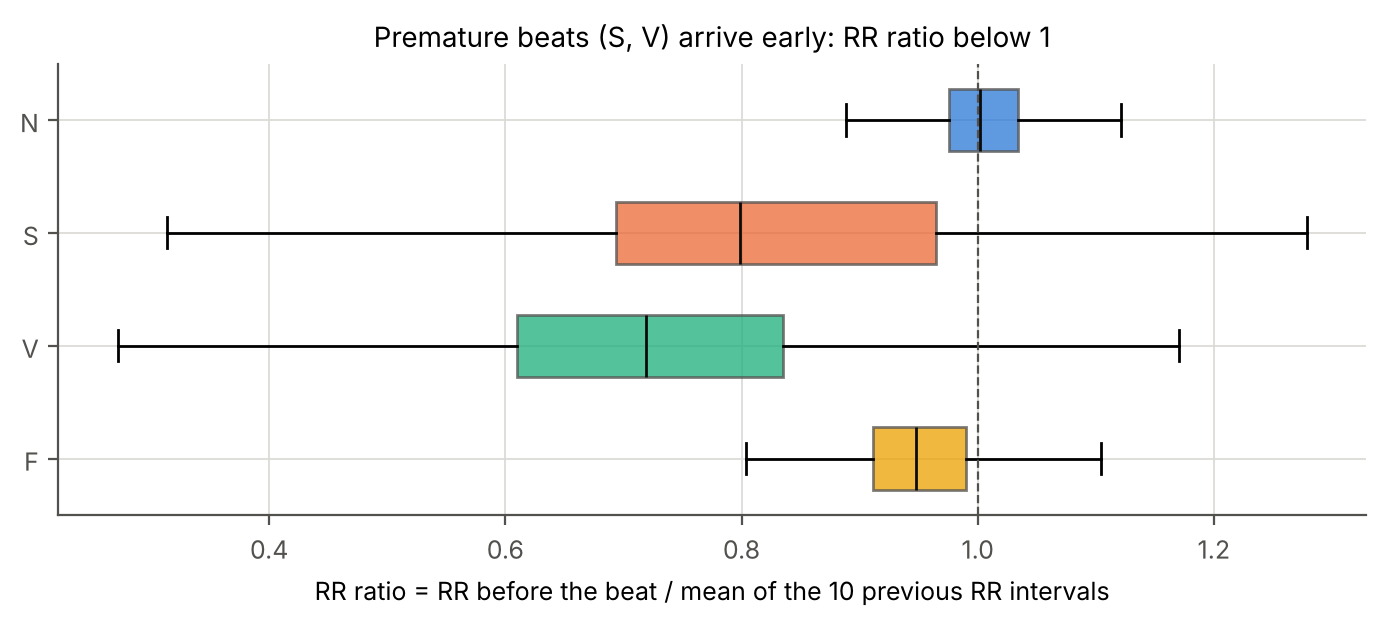
\includegraphics[width=0.65\textwidth]{fig_rr_ratio.png}
\caption{RR ratio per class in DS1. Values below 1 mean the beat came early.}
\label{fig:rr}
\end{figure}

\textbf{Class distribution.} N is about 90\,\% of every split (Figure~\ref{fig:classdist}). The test set has more S beats (3.7\,\%) than the training set (1.5\,\%), mostly because of record 232.

\begin{figure}[H]
\centering
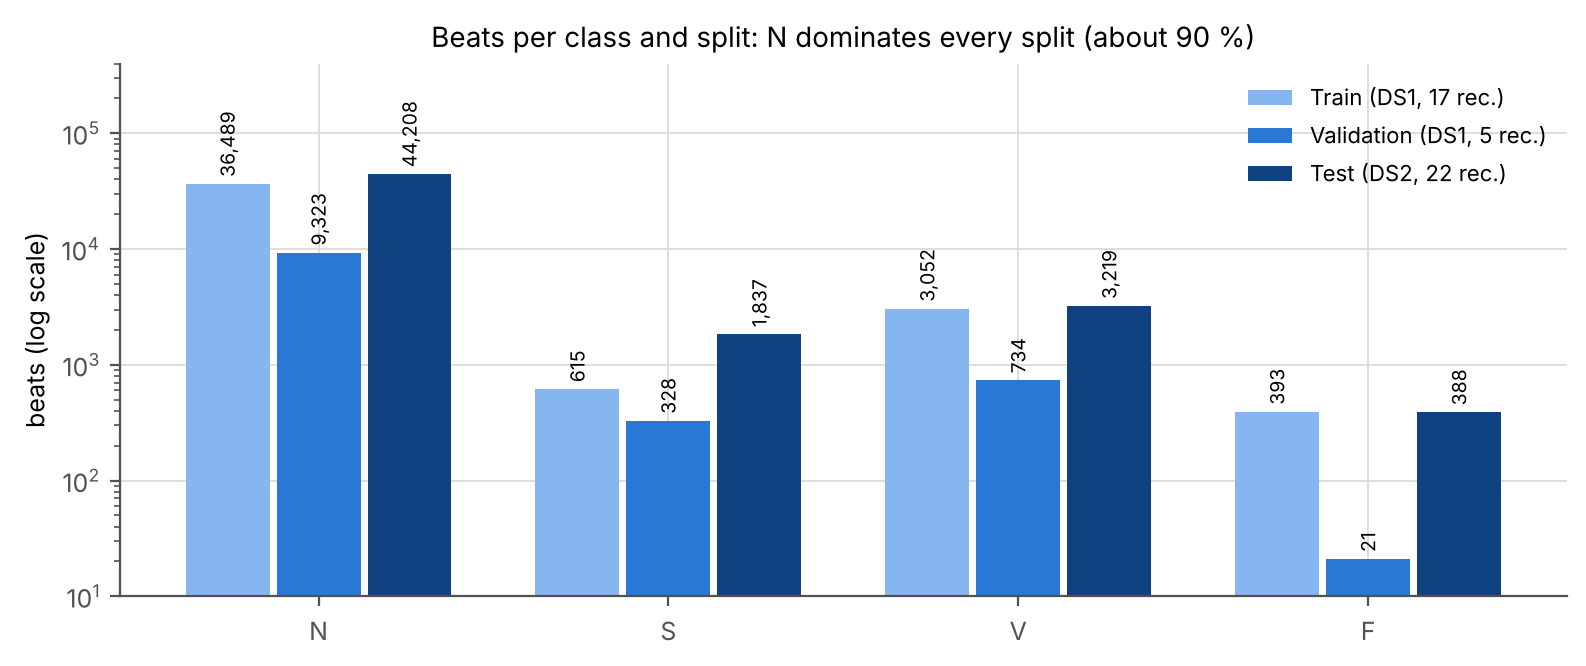
\includegraphics[width=0.75\textwidth]{fig_class_distribution.png}
\caption{Beats per class and split (log scale).}
\label{fig:classdist}
\end{figure}

\textbf{Record (patient) distribution.} Rare classes come from very few patients (Figure~\ref{fig:recdist}). In training, record 208 has 95\,\% of the F beats and record 209 has 62\,\% of the S beats. In the test set, record 213 has 93\,\% of the F beats and record 232 has 75\,\% of the S beats. So the model's ability to generalise is limited by the number of patients, not the number of beats.

\begin{figure}[H]
\centering
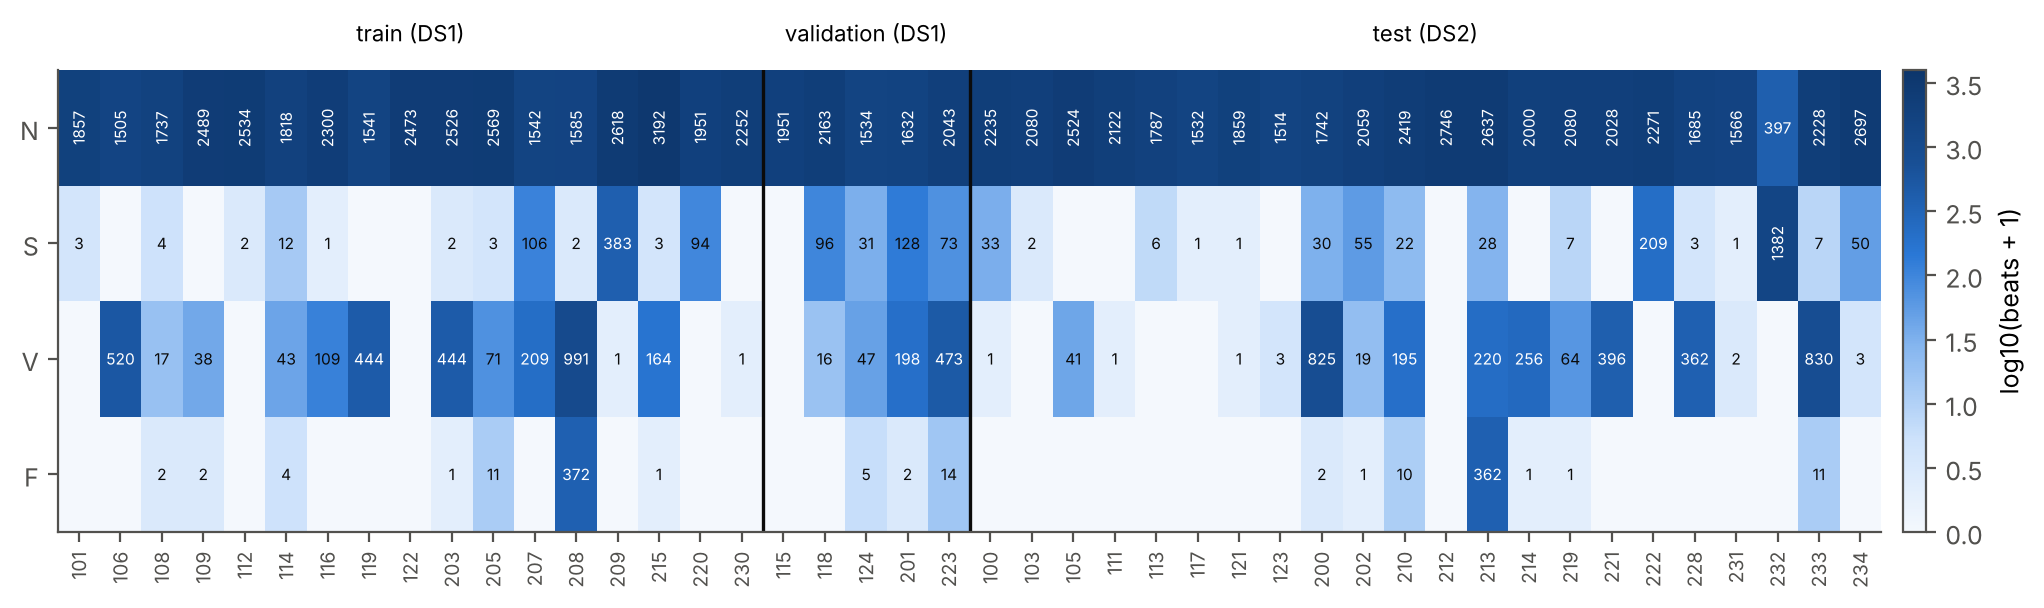
\includegraphics[width=\textwidth]{fig_record_distribution.png}
\caption{Beats per class in each record, grouped by split.}
\label{fig:recdist}
\end{figure}

\textbf{Signal amplitude.} The typical beat height differs 4.4 times between records, from 0.81~mV (record 222) to 3.59~mV (record 116) (Figure~\ref{fig:amp}). After scaling each record separately, all classes share the same value range.

\begin{figure}[H]
\centering
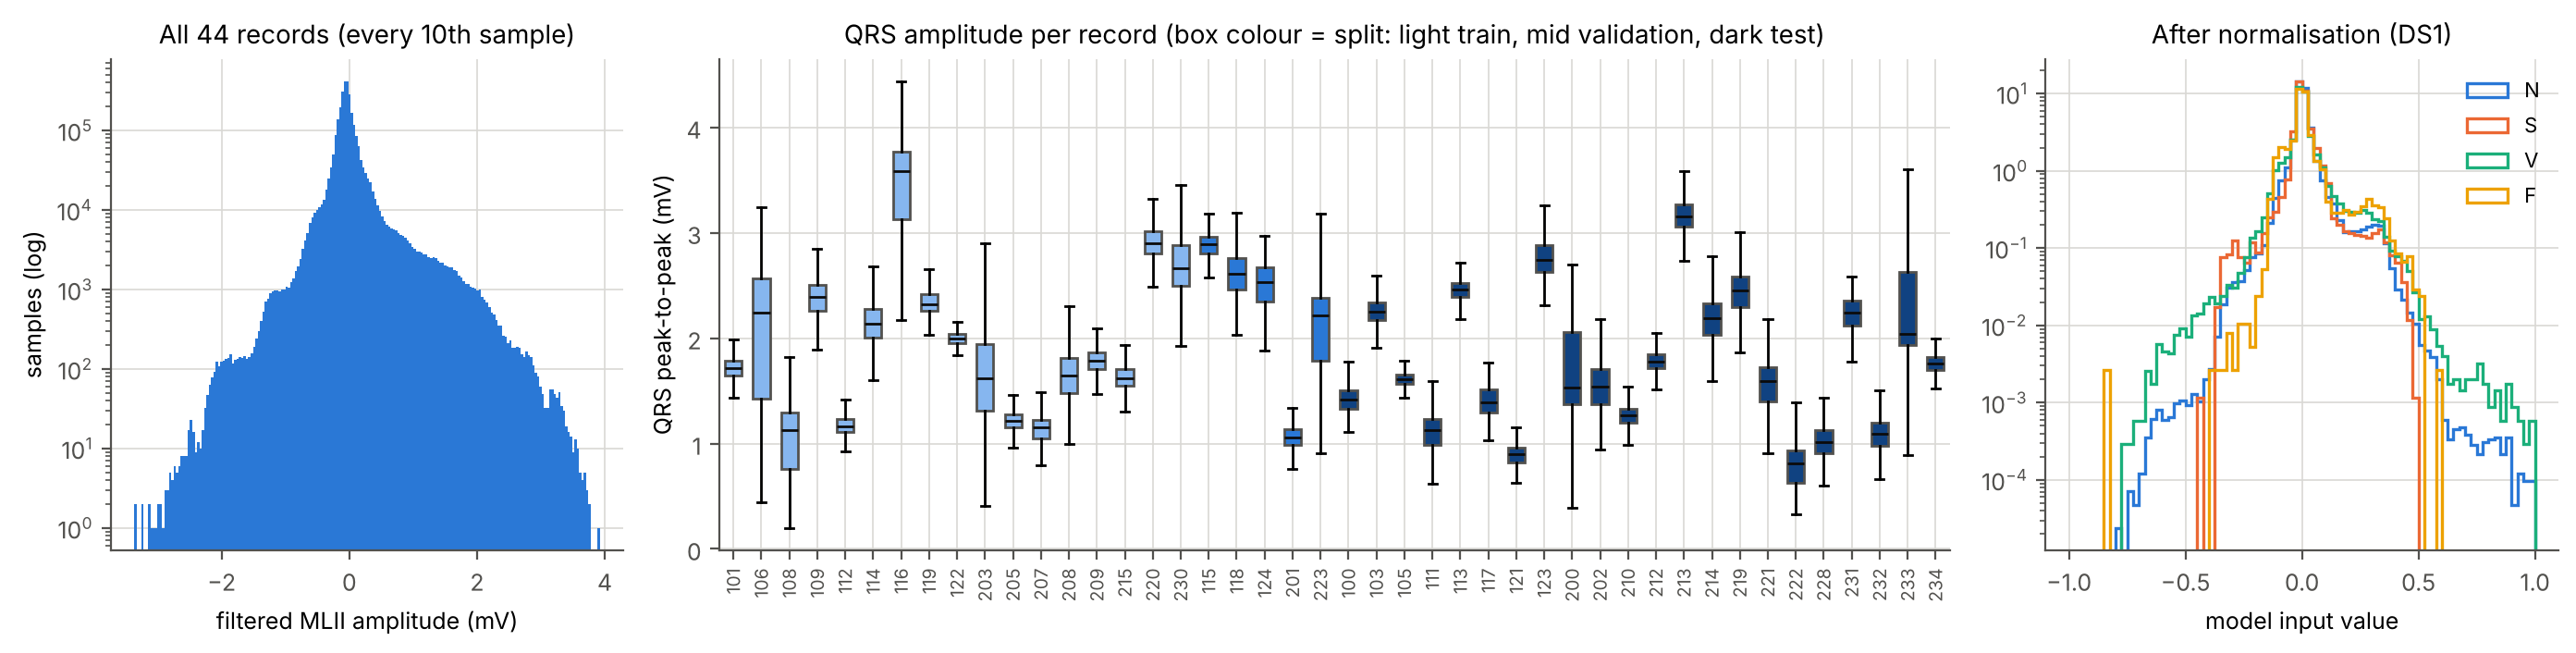
\includegraphics[width=\textwidth]{fig_amplitude.png}
\caption{Left: filtered signal values. Middle: beat height (QRS peak-to-peak) per record. Right: model input values per class after scaling.}
\label{fig:amp}
\end{figure}

\textbf{Noisy ECG.} Figure~\ref{fig:noise} adds the three noise types, and their mix, to a clean DS1 record at 12, 6 and 0~dB. We measure SNR the same way PhysioNet did when it built the noise database~\citep{physionet_nst}, based on the height of the QRS complex. Our first draft measured the signal as the average power of the whole ECG. That added between 2.8 and 11.7~dB less noise than intended, depending on the record (7.1~dB on average over DS1; \code{results/snr\_definition\_check\_ds1.csv}), so we changed it. Baseline wander is mostly removed by our filter, while electrode motion creates spikes that look like beats. Figure~\ref{fig:noise105} shows real noise in record 203.

\begin{figure}[H]
\centering
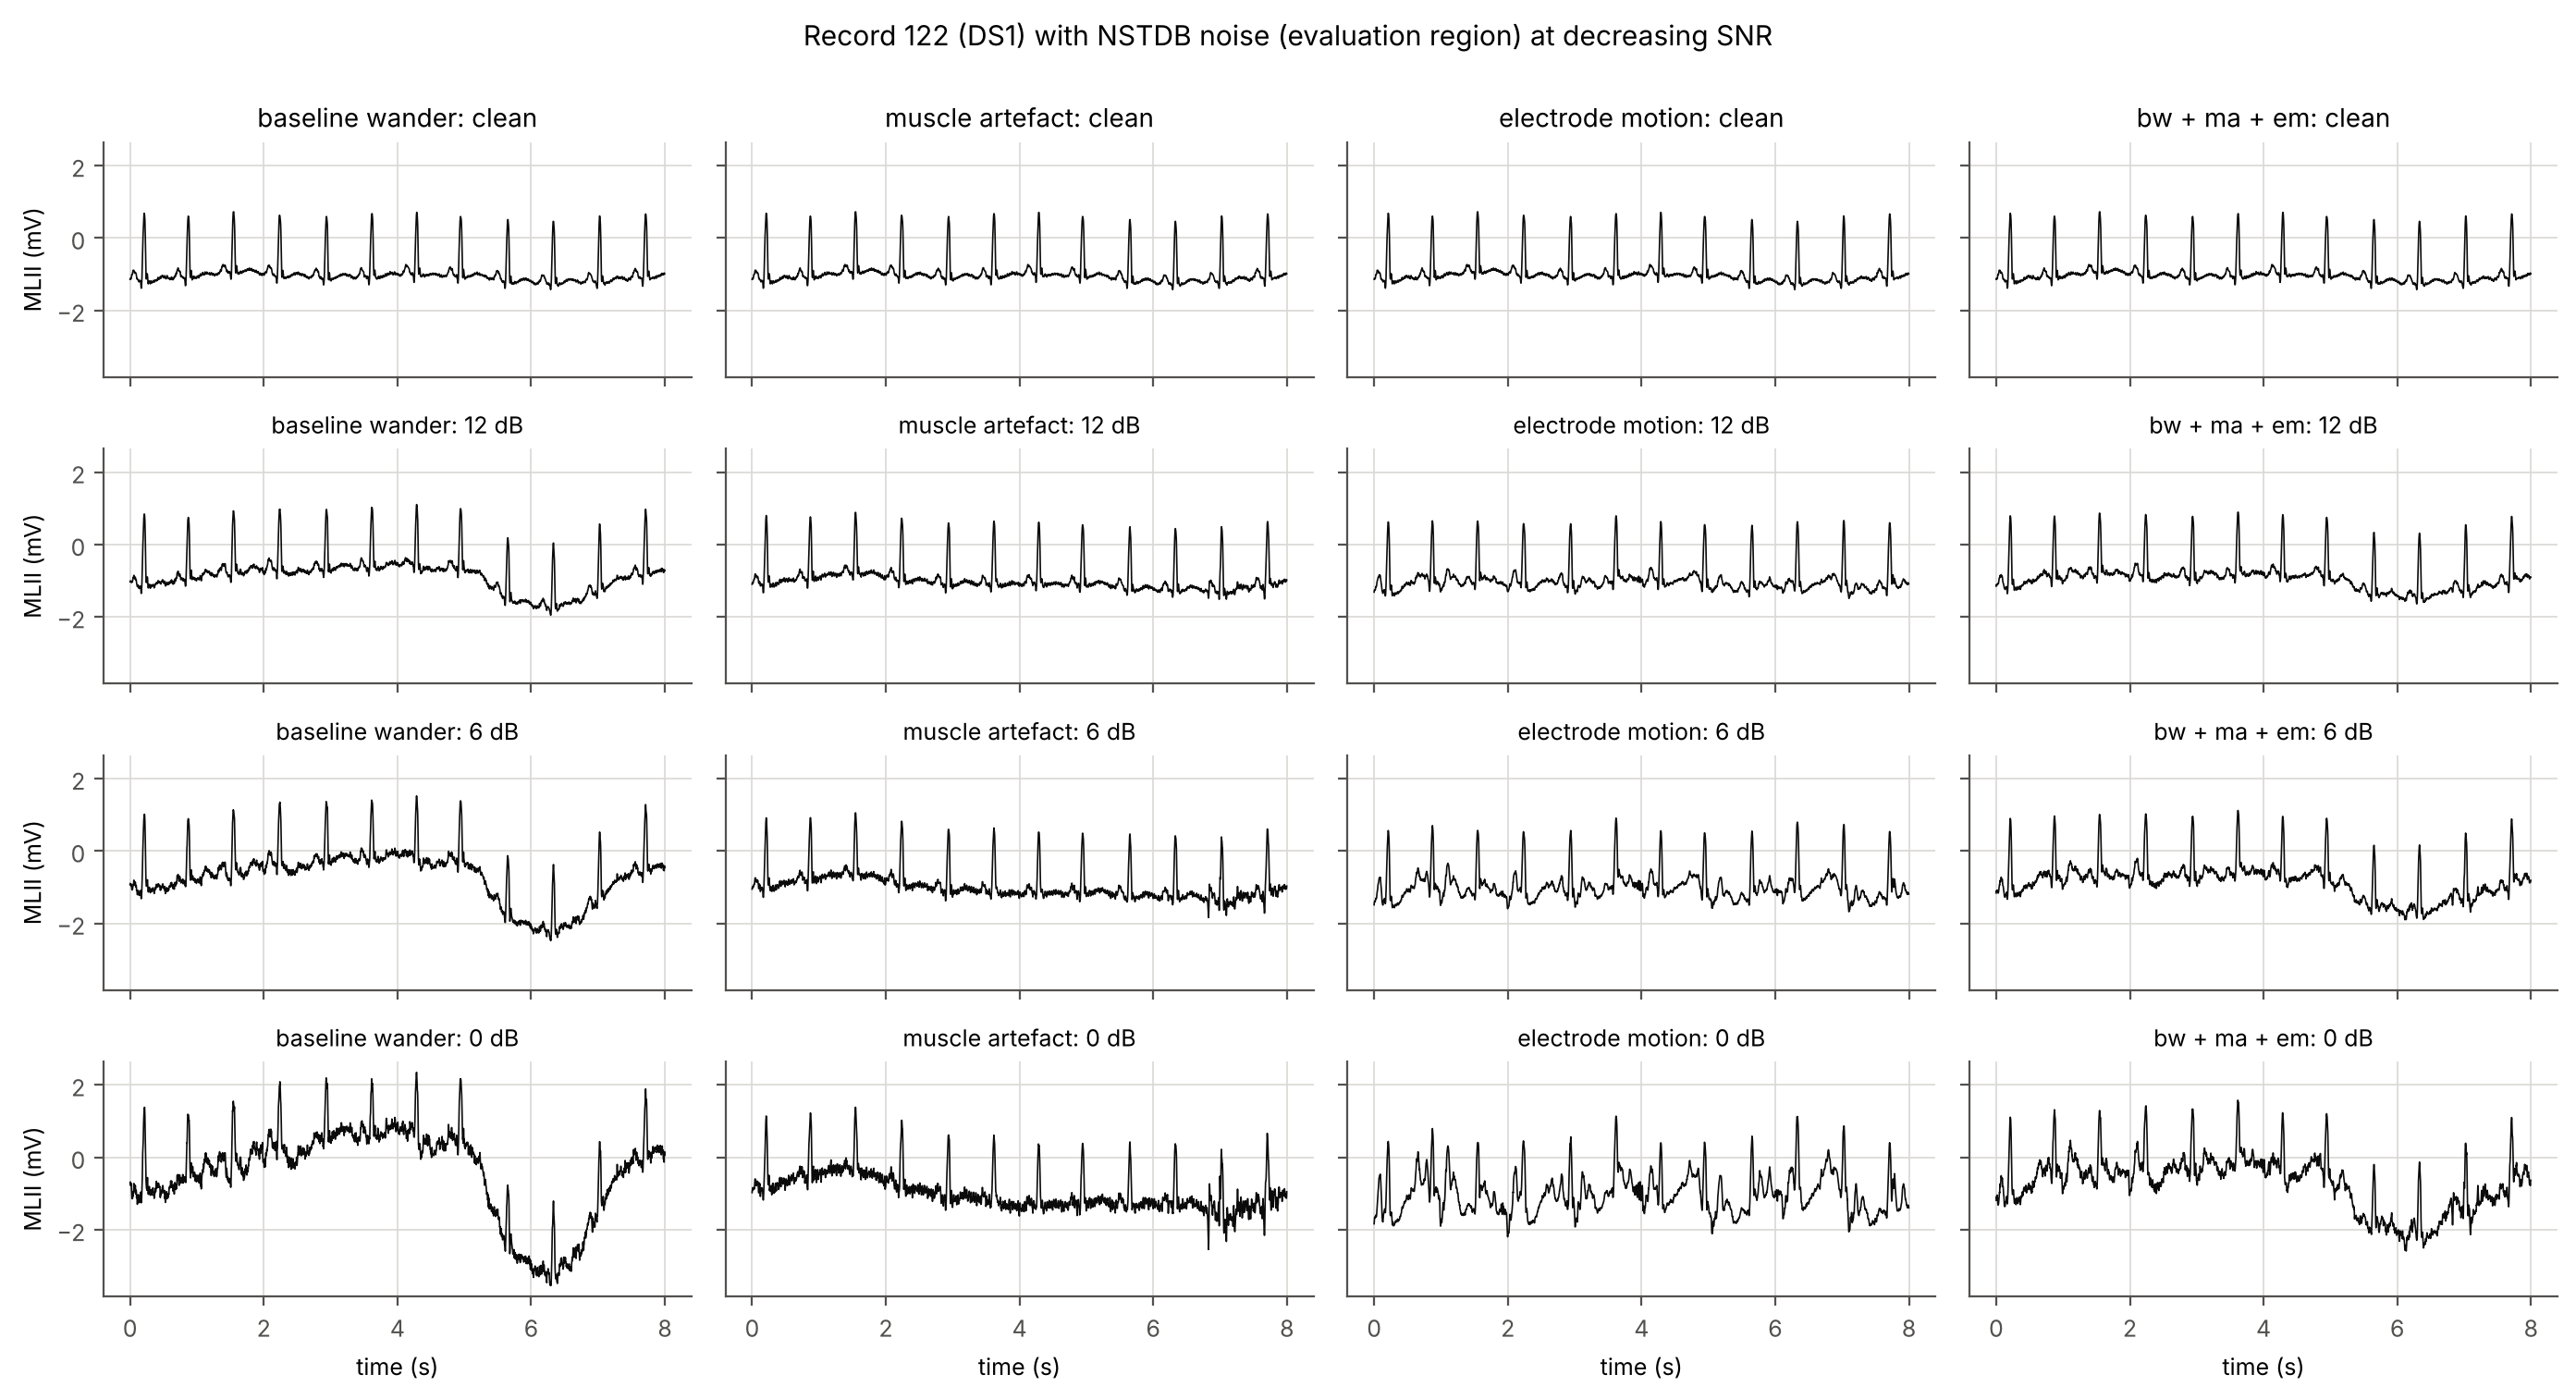
\includegraphics[width=0.92\textwidth]{fig_noise_examples.png}
\caption{DS1 record 122 with real noise added at decreasing SNR. The measured SNR matches the target within 0.01~dB.}
\label{fig:noise}
\end{figure}

\begin{figure}[H]
\centering
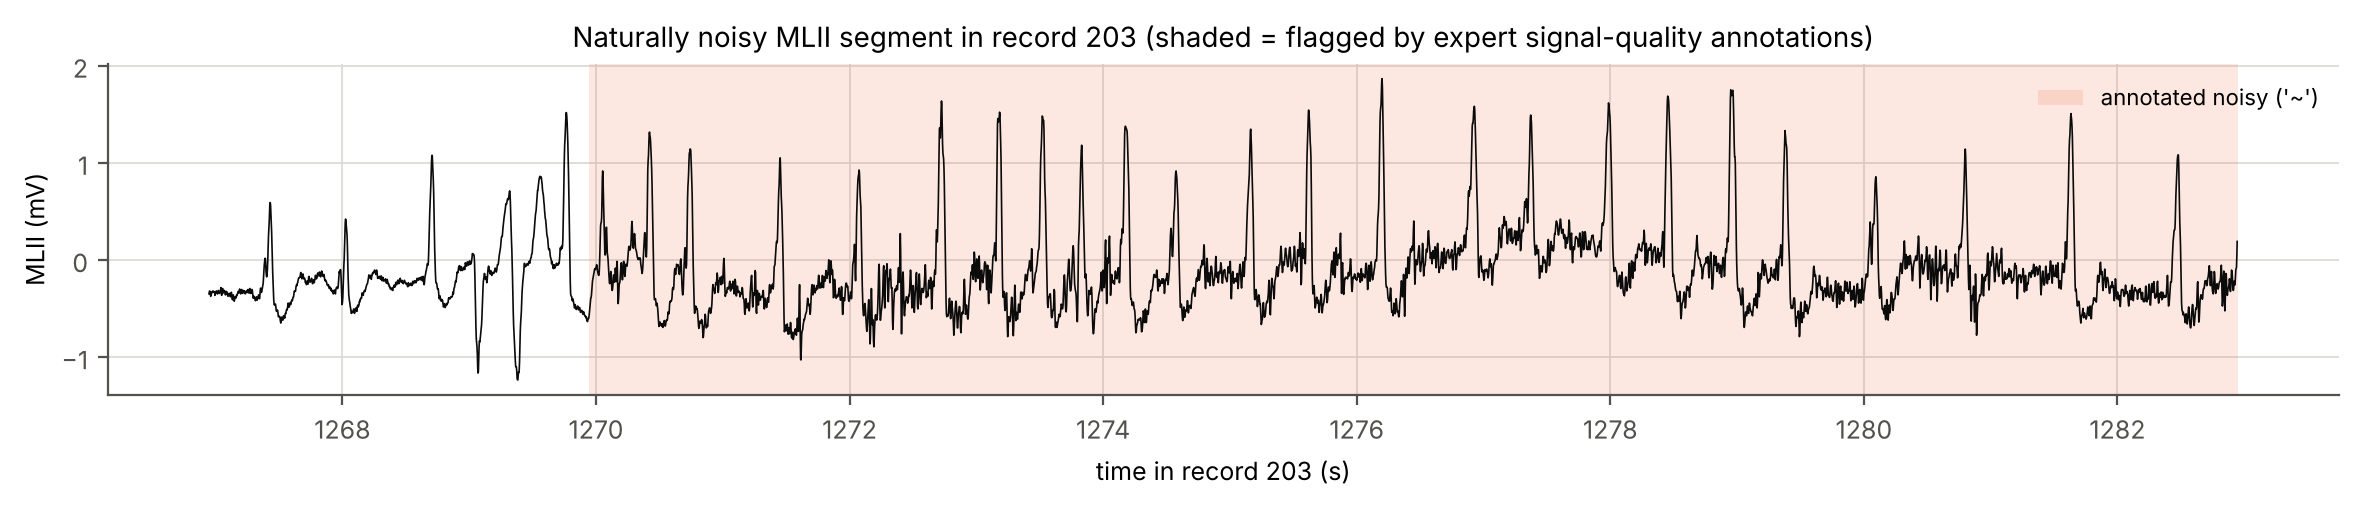
\includegraphics[width=\textwidth]{fig_noise_natural.png}
\caption{Real noise in DS1 record 203; the shaded part was marked as noisy by the experts.}
\label{fig:noise105}
\end{figure}

\subsection{Data Quality}

\begin{table}[H]
\centering
\small
\caption{Data-quality checks on the MLII lead of the 44 records (\code{results/data\_quality.csv}).}
\label{tab:quality}
\begin{tabularx}{\textwidth}{@{} >{\raggedright\arraybackslash}p{2.6cm} >{\raggedright\arraybackslash}p{4.0cm} L @{}}
\toprule
Check & How & What we found and did \\
\midrule
Missing data & Empty values; flat lines of 0.5~s or more & No missing values. Three flat lines, all in record 116, caused by saturation. Nothing to fill in. \\
Extreme amplitudes & Values at the recorder's limit; values above 5~mV & Only record 116 hits the limit (928 samples, 0.14\,\%), during its very tall beats. Clipping in preprocessing handles this. \\
Corrupted segments & Time marked noisy by the experts & 23.1~min in total (1.7\,\%). Most in records 105 (14.4\,\%), 203 (12.7\,\%) and 108 (10.9\,\%). We keep these beats: their labels are valid and a wearable must cope with noise. \\
Possible noisy regions & How similar each normal beat is to the record's typical beat (low if correlation $< 0.8$) & Highest in 108 (50.9\,\%), 222 and 117 (about 30\,\%). Agrees fairly well with the experts' notes (Spearman 0.62) (Figure~\ref{fig:quality}). \\
Class imbalance & Counts per split & N is 89--90\,\% of every split, F 0.2--1.0\,\%. See Section~\ref{sec:imbalance}. \\
Differences between recordings & Beat height, heart rate, class mix & Beat height 0.81--3.59~mV, heart rate 50--112~bpm, from N-only records to 78\,\% S (record 232). We scale each record separately and split by record. \\
Differences between channels & Lead names; correlation with MLII & The second lead changes between records (V1, V2, V4, V5) and its correlation with MLII ranges from $-0.83$ to $0.93$ (Figure~\ref{fig:channels}). We use MLII only. \\
\bottomrule
\end{tabularx}
\end{table}

\begin{figure}[H]
\centering
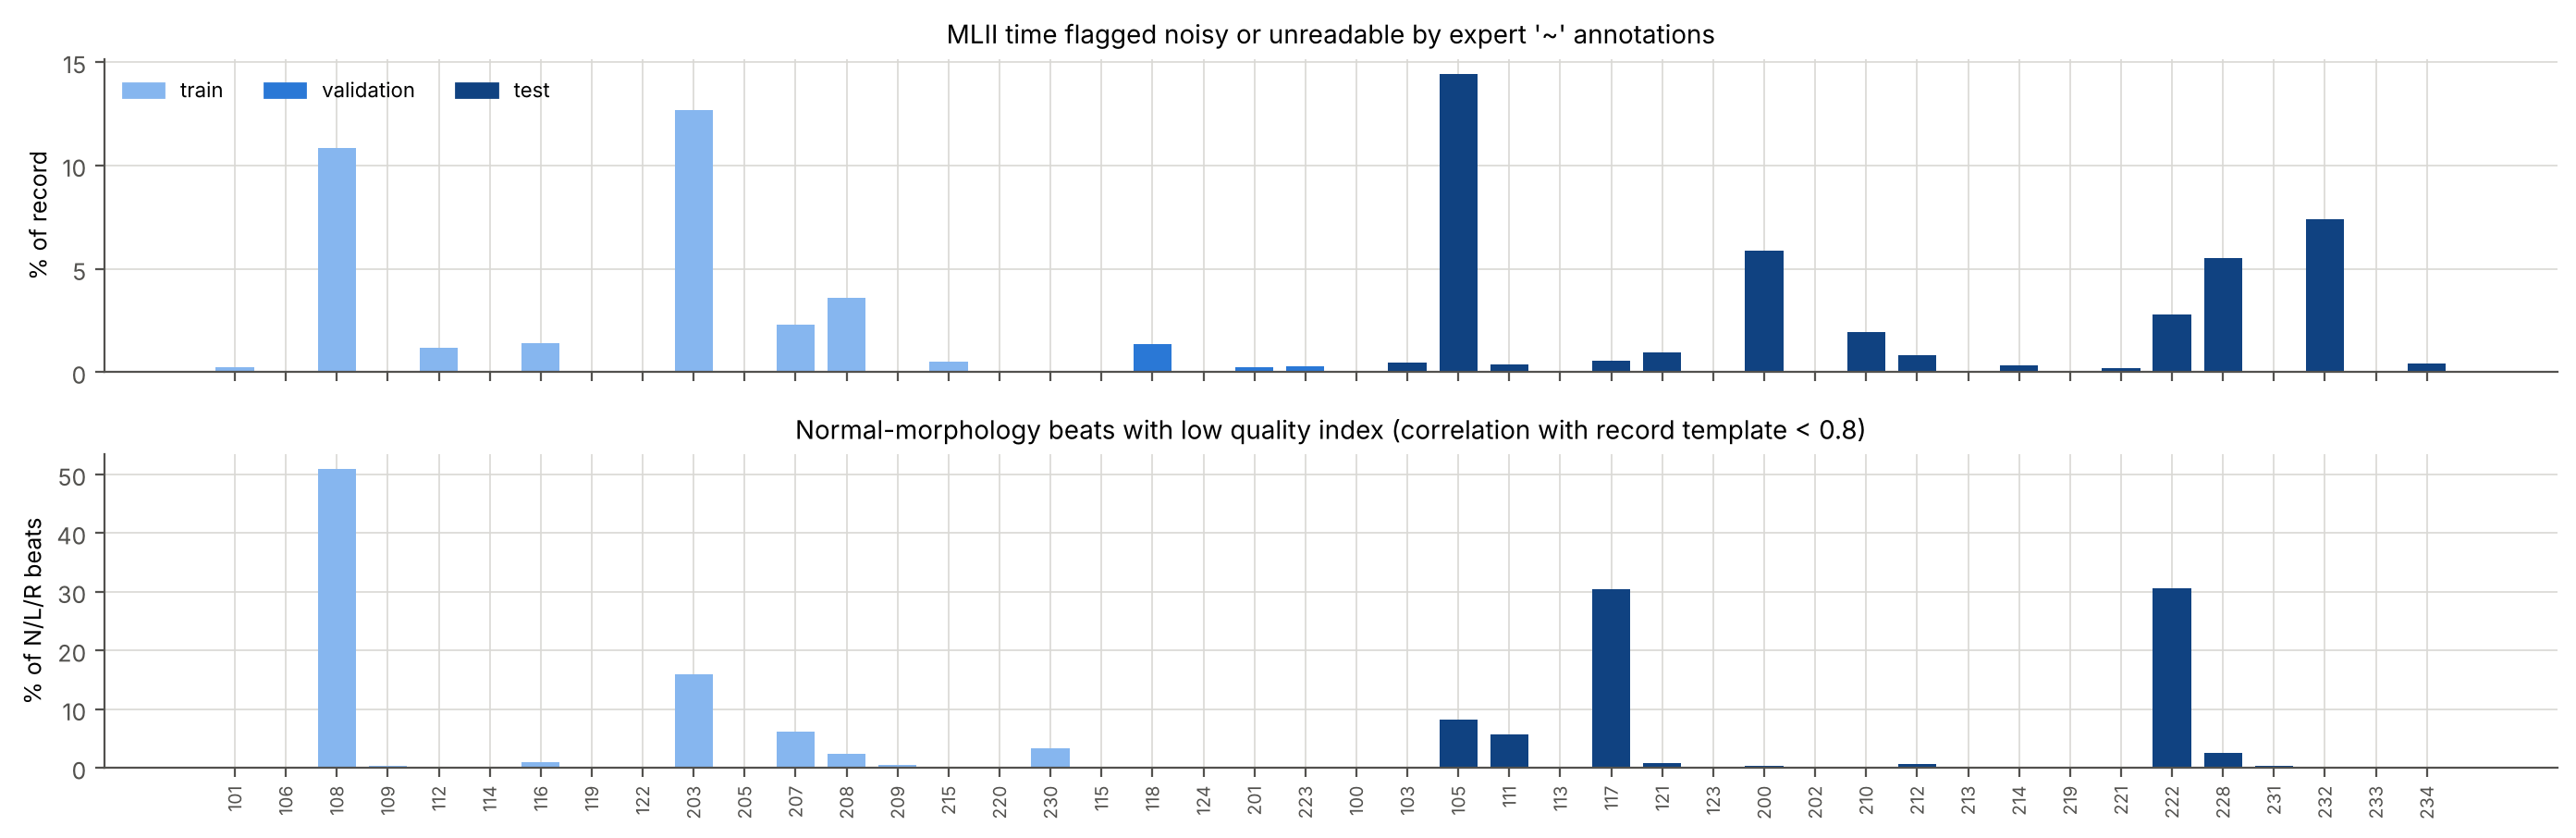
\includegraphics[width=\textwidth]{fig_data_quality.png}
\caption{Per record: share of time marked noisy (top) and share of normal beats with low similarity (bottom).}
\label{fig:quality}
\end{figure}

\begin{figure}[H]
\centering
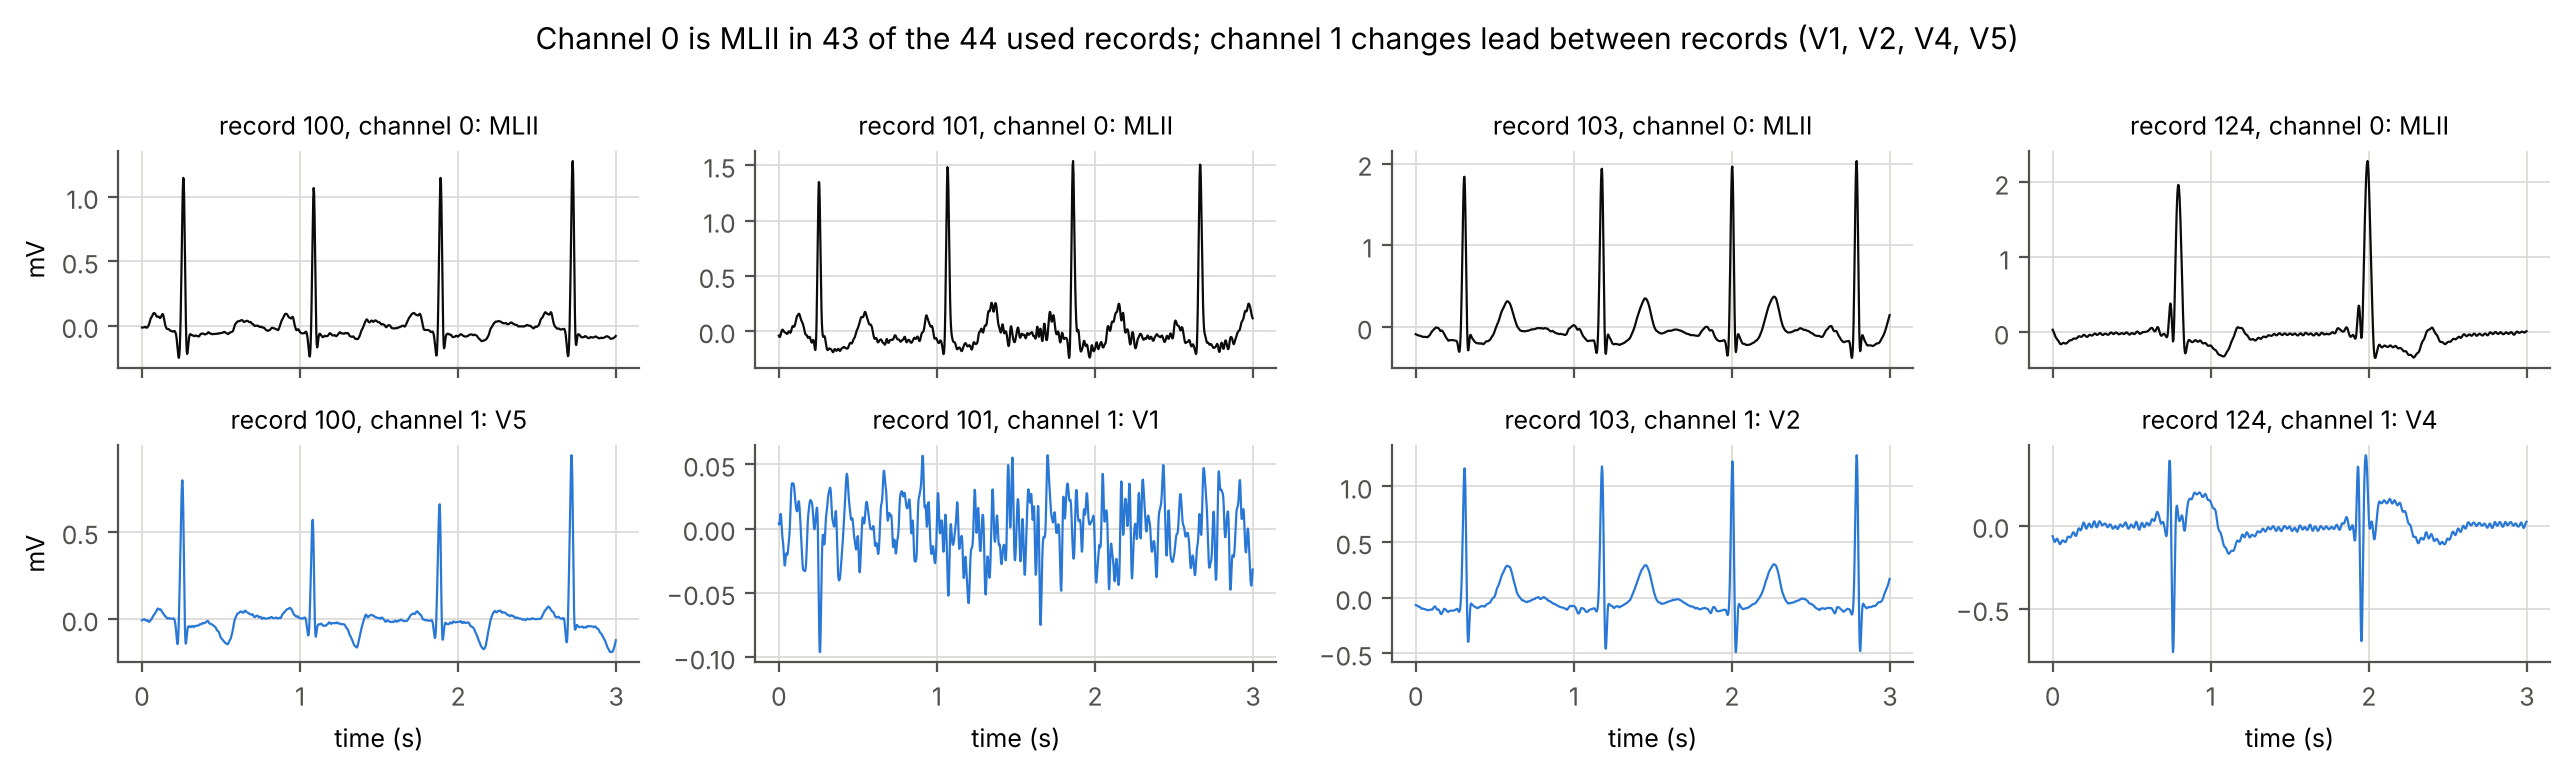
\includegraphics[width=\textwidth]{fig_channels.png}
\caption{Channel 0 (MLII) and channel 1 for four records. Channel 1 is a different lead in each.}
\label{fig:channels}
\end{figure}

\subsection{Leakage Analysis}
\label{sec:leakage}

Data leakage means that information from the test data reaches training or model selection, so the reported score is better than what we would get on new patients.

\textbf{Why a random beat split is misleading.} One record holds 1,500--3,400 beats from the same person, with the same electrodes and the same beat shape. If beats from one record end up in both training and test sets, the model can recognise the \emph{patient} instead of the beat type: almost every test beat has a near-copy in training. The score then says nothing about a new wearer.

\textbf{Our own evidence (DS1 only).} We ran the same simple classifier (1-nearest neighbour) twice on DS1 (Table~\ref{tab:leak}, Figure~\ref{fig:leak}). With a random 80/20 beat split, 96.5\,\% of test beats find their closest match in the same record, and macro F1 is 0.875. When five whole records are held out, macro F1 drops to 0.492 and F recall from 0.66 to 0.05. Accuracy hides most of this (0.987 against 0.923) because N dominates.

\begin{table}[H]
\centering
\small
\caption{Leakage test on DS1 (\code{results/leakage\_experiment.csv}). DS2 was not used.}
\label{tab:leak}
\setlength{\tabcolsep}{4.5pt}
\begin{tabular}{@{} l r r r r r r r @{}}
\toprule
Split & Accuracy & Macro F1 & N rec. & S rec. & V rec. & F rec. & Match in same rec. \\
\midrule
Random beat split (leaky) & 0.987 & 0.875 & 0.995 & 0.820 & 0.966 & 0.663 & 96.5\,\% \\
Record split (17 $\rightarrow$ 5 records) & 0.923 & 0.492 & 0.983 & 0.381 & 0.425 & 0.048 & 0.0\,\% \\
\bottomrule
\end{tabular}
\end{table}

\begin{figure}[H]
\centering
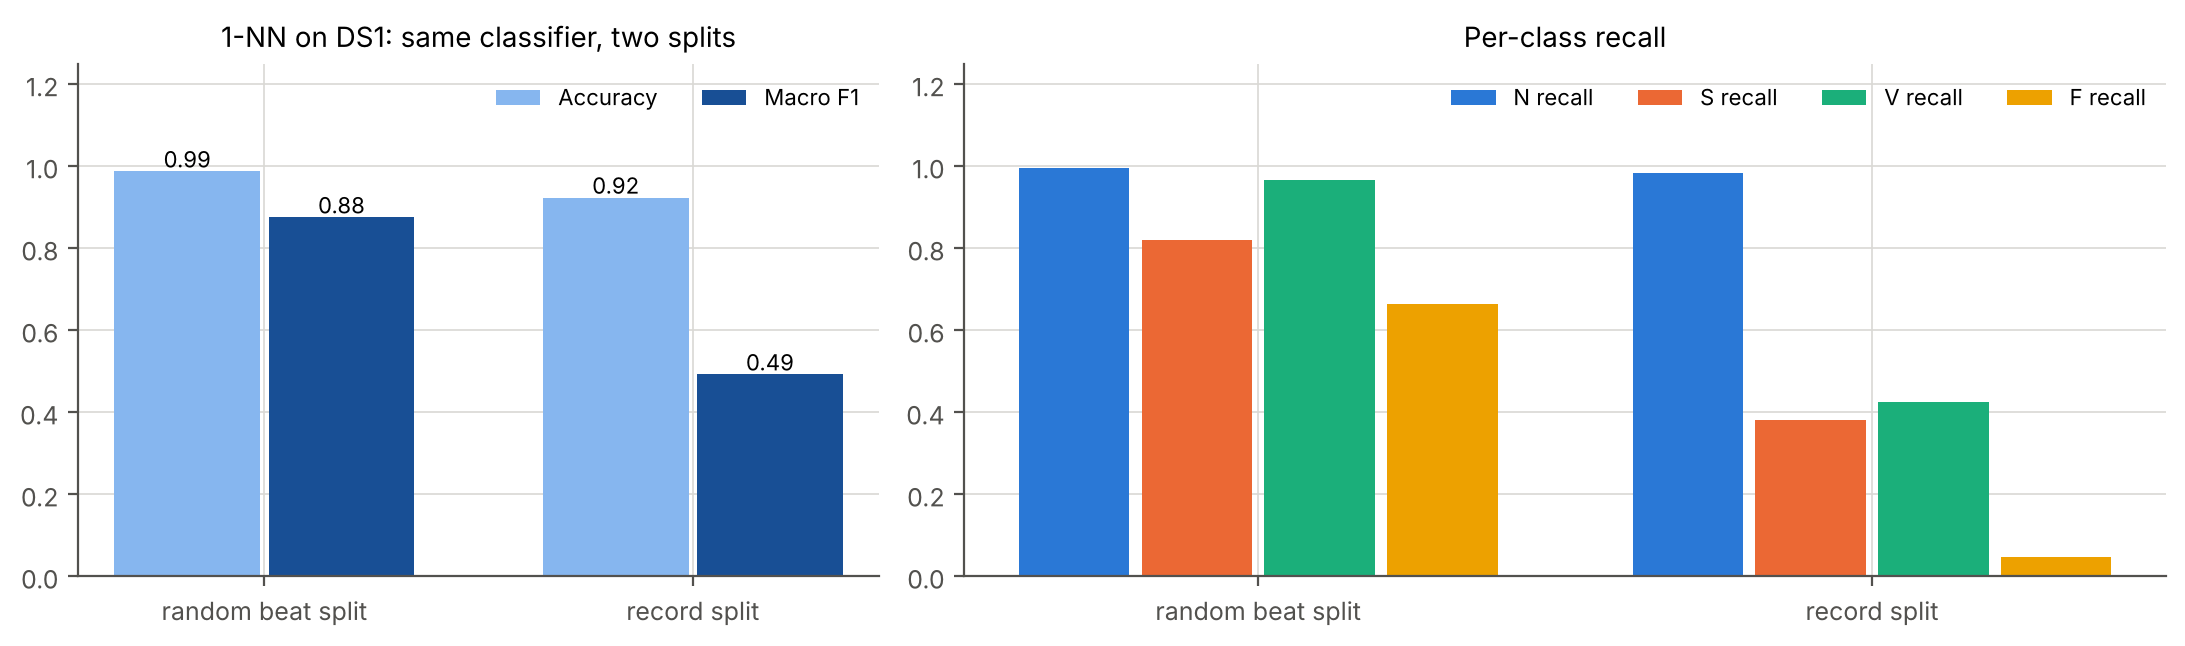
\includegraphics[width=0.9\textwidth]{fig_leakage.png}
\caption{The same classifier with a random beat split and with a record split.}
\label{fig:leak}
\end{figure}

\textbf{How we prevent leakage.}
\begin{itemize}
  \item \textbf{Split by record.} Each record is in exactly one split. The code stops with an error if the training, validation and test lists overlap, or if they do not match DS1 and DS2.
  \item \textbf{DS2 is used once.} It is processed by the same code but saved to its own file, which only the final evaluation reads. No choice in this report used DS2.
  \item \textbf{No shared statistics.} The filter is fixed, and each record is scaled using only its own signal, without labels.
  \item \textbf{Same patient in two records.} Records 201 (DS1) and 202 (DS2) are the same person. We keep the standard split, as the assignment asks, but put 201 in validation so no training beat comes from a test patient. We note this as a limitation.
  \item \textbf{Noise.} Real noise is never used for training. Only the second half of each noise recording is used for testing; the first half is kept aside.
\end{itemize}

% =====================================================================
\section{Data Preparation}
% =====================================================================

Every N, S, V and F beat becomes a $2 \times 256$ array using \code{src/prepare\_data.py}. All settings are in \code{configs/data.yaml}.

\subsection{Record Selection}

\begin{table}[H]
\centering
\small
\caption{Records in each split.}
\label{tab:records}
\begin{tabularx}{\textwidth}{@{} l L c L @{}}
\toprule
Split & Records & Count & Used for \\
\midrule
Train (DS1) & 101, 106, 108, 109, 112, 114, 116, 119, 122, 203, 205, 207, 208, 209, 215, 220, 230 & 17 & Fitting the model \\
Validation (DS1) & 115, 118, 124, 201, 223 & 5 & Choosing models and settings \\
Test (DS2) & 100, 103, 105, 111, 113, 117, 121, 123, 200, 202, 210, 212, 213, 214, 219, 221, 222, 228, 231, 232, 233, 234 & 22 & Final evaluation, once \\
Excluded & 102, 104, 107, 217 (paced) & 4 & Not used \\
\bottomrule
\end{tabularx}
\end{table}

We chose validation records that together contain all four classes. Record 208 stays in training because it holds 90\,\% of the DS1 F beats. The downside is that validation has only 21 F beats, so F scores on validation will be unstable.

\subsection{ECG Channel Selection}

We use the \textbf{MLII} lead only. It is present in all 44 records, the beats are clear in it, and a single lead is closest to what a wearable records. The second channel uses a different lead in different records, which would give the model inconsistent input. We find MLII by its name, not its position, because record 114 stores it in channel~1. If a record has no MLII it is skipped; this only happens for the paced records 102 and 104, which are excluded anyway.

\subsection{Beat Extraction}

\begin{itemize}
  \item \textbf{Beat positions:} taken from the expert annotations, so we do not run our own beat detector. A real wearable would need one; the time-shift augmentation (Section~\ref{sec:aug}) prepares the model for small position errors.
  \item \textbf{Window:} 450 samples before and 270 after the beat at 360~Hz (1.25~s and 0.75~s), so 720 samples in total.
  \item \textbf{Why this window:} at heart rates above 48~bpm it also contains the previous beat, so the model can see whether the beat came early. It covers the whole current beat as well.
  \item \textbf{Final input:} the window is resampled to 256 samples (128~Hz), with the beat at sample 160. A second channel holds the RR ratio. Input size: $2 \times 256$.
\end{itemize}

\subsection{Signal Preprocessing}

\begin{figure}[H]
\centering
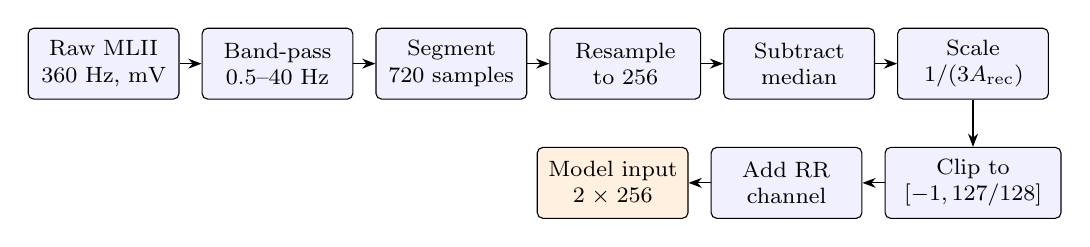
\begin{tikzpicture}[node distance=2.8mm, box/.style={draw, rounded corners=2pt, fill=blue!6, align=center, font=\footnotesize, minimum height=9mm, text width=16.8mm}, >=Stealth]
\node[box] (a) {Raw MLII\\360~Hz, mV};
\node[box, right=of a] (b) {Band-pass\\0.5--40~Hz};
\node[box, right=of b] (c) {Segment\\720 samples};
\node[box, right=of c] (d) {Resample\\to 256};
\node[box, right=of d] (e) {Subtract\\median};
\node[box, right=of e] (f) {Scale\\$1/(3A_{\text{rec}})$};
\node[box, below=6mm of f, text width=20mm] (g) {Clip to\\$[-1, 127/128]$};
\node[box, left=of g] (h) {Add RR\\channel};
\node[box, left=of h, fill=orange!12] (i) {Model input\\$2 \times 256$};
\draw[->] (a) -- (b); \draw[->] (b) -- (c); \draw[->] (c) -- (d); \draw[->] (d) -- (e); \draw[->] (e) -- (f);
\draw[->] (f) -- (g); \draw[->] (g) -- (h); \draw[->] (h) -- (i);
\end{tikzpicture}
\caption{Preprocessing steps, the same for every split.}
\label{fig:pipeline}
\end{figure}

\begin{table}[H]
\centering
\small
\caption{Preprocessing steps in order and why each is needed.}
\label{tab:prep}
\begin{tabularx}{\textwidth}{@{} >{\raggedright\arraybackslash}p{2.4cm} >{\raggedright\arraybackslash}p{4.6cm} L @{}}
\toprule
Step & What we do & Why \\
\midrule
1. Filter & Butterworth band-pass 0.5--40~Hz, run forwards and backwards & Removes slow drift and high-frequency noise but keeps the beat. Running it both ways keeps the peak in place (a device would use a one-way filter). \\
2. Segment & Cut 720 samples around each beat & The model needs a fixed-size input. \\
3. Resample & 360~Hz $\rightarrow$ 128~Hz (720 $\rightarrow$ 256 samples) & 2.8 times less data and computation; 128~Hz still covers the 40~Hz content. \\
4. Centre & Subtract the window median & Puts every window around zero. \\
5. Scale & Divide by $3 \times A_{\text{rec}}$, where $A_{\text{rec}}$ is the typical beat peak of the record & Removes height differences between patients but keeps V beats taller than N beats within a patient. \\
6. Clip & Limit values to $[-1, 127/128]$ & Matches the 8-bit input of the MAX78002 and limits artefact spikes. \\
7. RR channel & Add the RR ratio as a second channel & Gives the timing information that shape alone does not carry (Figure~\ref{fig:rr}). \\
\bottomrule
\end{tabularx}
\end{table}

\textbf{How we chose the scaling (DS1 only).} The first draft divided by $2 \times$ the signal value at the beat annotation. On DS1 this cut off the peaks of 4.3\,\% of V beats, and of 83.5\,\% of the V beats in record 215, so the shape that identifies them was lost (\code{results/normalization\_choice\_ds1.csv}). Using the beat peak within $\pm 50$~ms and a factor of 3 reduces this to a single V beat (0.03\,\%), while a normal beat still uses 43 of the 127 positive 8-bit levels. In DS2, record 228 still has some clipped V beats (157 of 362). We report this but do not tune on it, because DS2 must not influence our choices; it is picked up again in the error analysis of Task 2.

\begin{figure}[H]
\centering
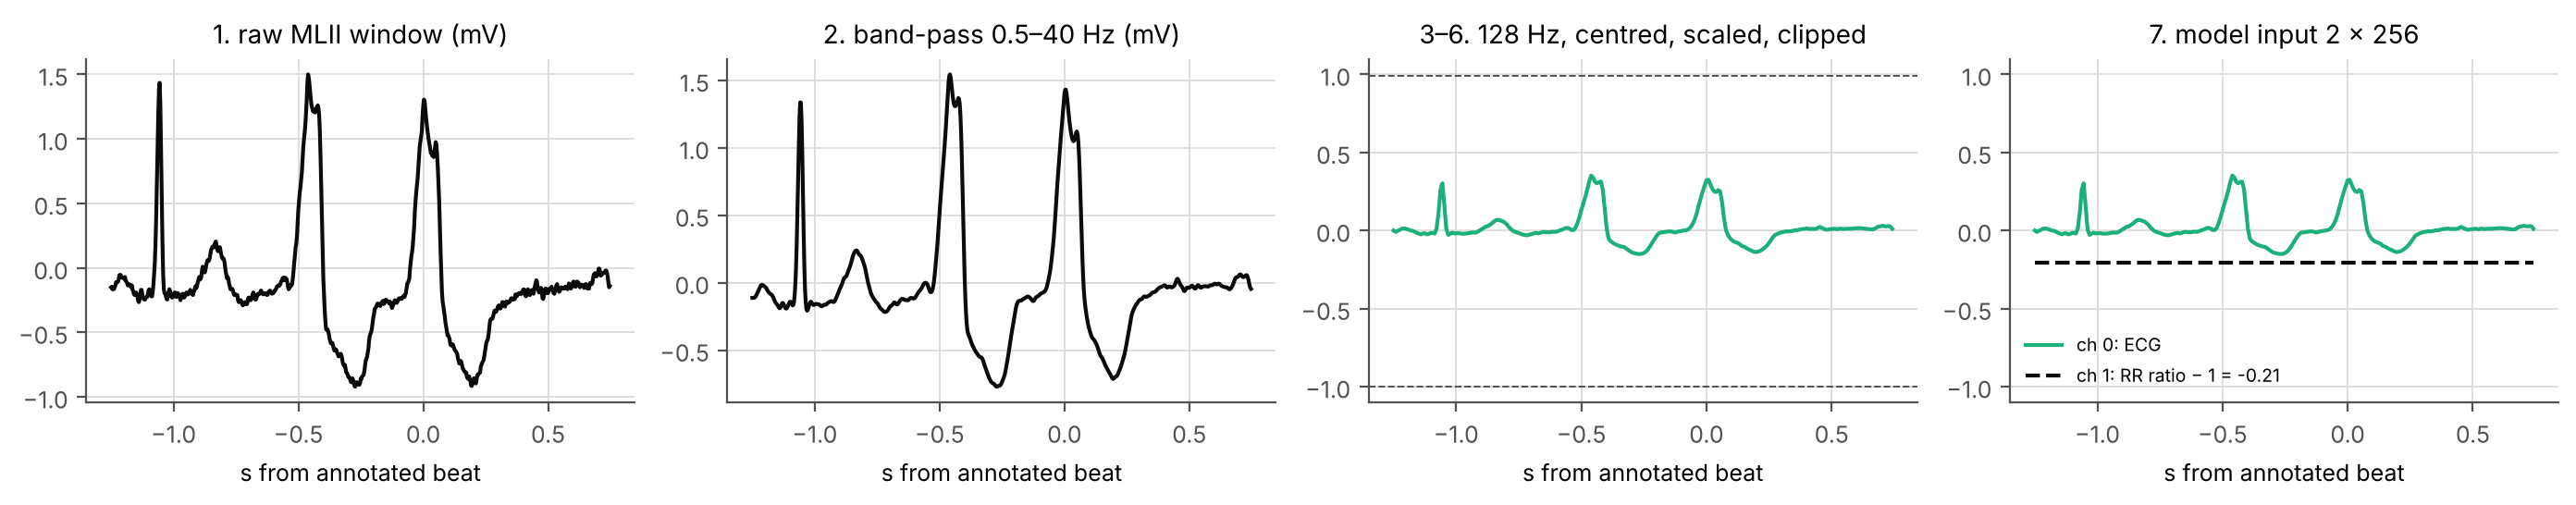
\includegraphics[width=\textwidth]{fig_preprocessing_steps.png}
\caption{One V beat from record 208 through the steps. Dashed lines in panel 3 are the clipping limits.}
\label{fig:prepsteps}
\end{figure}

\subsection{Label Preparation}

\begin{table}[H]
\centering
\small
\caption{Mapping from MIT-BIH labels to our classes (class numbers N = 0, S = 1, V = 2, F = 3).}
\label{tab:labels}
\begin{tabularx}{\textwidth}{@{} l L l @{}}
\toprule
MIT-BIH symbol & Meaning & Class \\
\midrule
\code{N}, \code{L}, \code{R}, \code{e}, \code{j} & Normal, left and right bundle branch block, atrial escape, nodal escape & N \\
\code{A}, \code{a}, \code{J}, \code{S} & Atrial premature, aberrated atrial premature, nodal premature, supraventricular premature & S \\
\code{V}, \code{E} & Premature ventricular contraction, ventricular escape & V \\
\code{F} & Fusion of ventricular and normal beat & F \\
\code{/}, \code{f}, \code{Q} & Paced, fusion of paced and normal, unclassifiable & Excluded \\
\code{+ \textasciitilde{} | x ! [ ] "} & Rhythm, signal quality, artefact and other notes & Not beats \\
\bottomrule
\end{tabularx}
\end{table}

\subsection{Class Imbalance}
\label{sec:imbalance}

\begin{table}[H]
\centering
\small
\caption{Class shares per split (\code{results/class\_counts.csv}) and training class weights (\code{results/class\_weights.csv}).}
\label{tab:imbalance}
\begin{tabular}{@{} l r r r r l @{}}
\toprule
 & N & S & V & F & N : S : V : F \\
\midrule
Train & 89.99\,\% & 1.52\,\% & 7.53\,\% & 0.97\,\% & 92.8 : 1.6 : 7.8 : 1 \\
Validation & 89.59\,\% & 3.15\,\% & 7.05\,\% & 0.20\,\% & 444 : 15.6 : 35 : 1 \\
Test & 89.04\,\% & 3.70\,\% & 6.48\,\% & 0.78\,\% & 114 : 4.7 : 8.3 : 1 \\
\midrule
Class weight & 0.18 & 1.41 & 0.63 & 1.77 & \\
\bottomrule
\end{tabular}
\end{table}

\textbf{Our choice: class weights in the loss.} Each class gets the weight $w_c = (n_{\max}/n_c)^{0.5}$, scaled to an average of 1 and computed on the training split only. Taking the square root means an F beat counts about 10 times as much as an N beat, instead of 93 times. Full weights would let the few F beats from one patient dominate training. We also choose models by macro F1, which rewards the rare classes.

Why not the other options:
\begin{itemize}
  \item \textbf{Oversampling or balanced batches} would repeat the F beats of one patient (record 208) many times, so the model would memorise that patient.
  \item \textbf{Undersampling} N would throw away most of the data and many patients.
  \item \textbf{Focal loss}~\citep{lin2017focal} adds a setting we would have to tune on a small validation set. It is tested in Task 2, together with \textbf{no balancing} as a reference (Section~\ref{sec:selection}).
  \item \textbf{Adjusting decision thresholds} per class would also be tuned on only 21 validation F beats, so we do not use it now.
\end{itemize}

\subsection{Data Augmentation}
\label{sec:aug}

During training only, each beat is randomly changed in four ways (\code{src/dataset.py}). Each change is applied with probability 0.5 and affects only the ECG channel. Validation and test data are never changed. Sizes are relative to the scaled signal, where a normal beat peak is about 0.33.

\begin{table}[H]
\centering
\small
\caption{Augmentation, training split only.}
\label{tab:aug}
\begin{tabularx}{\textwidth}{@{} l l L @{}}
\toprule
Change & Range & Simulates \\
\midrule
Amplitude scaling & factor 0.8--1.2 & Different electrode contact \\
Time shift & $\pm 5$ samples ($\pm 39$~ms) & Small errors of a beat detector \\
Gaussian noise & $\sigma$ 0.003--0.02 & High-frequency noise \\
Baseline wander & slow sine, 0.15--0.5~Hz, up to 0.07 & Breathing and electrode drift \\
\bottomrule
\end{tabularx}
\end{table}

We do not use the real NSTDB noise for training, so the noise test in Task 2 measures how the model handles noise it has never seen.

\begin{figure}[H]
\centering
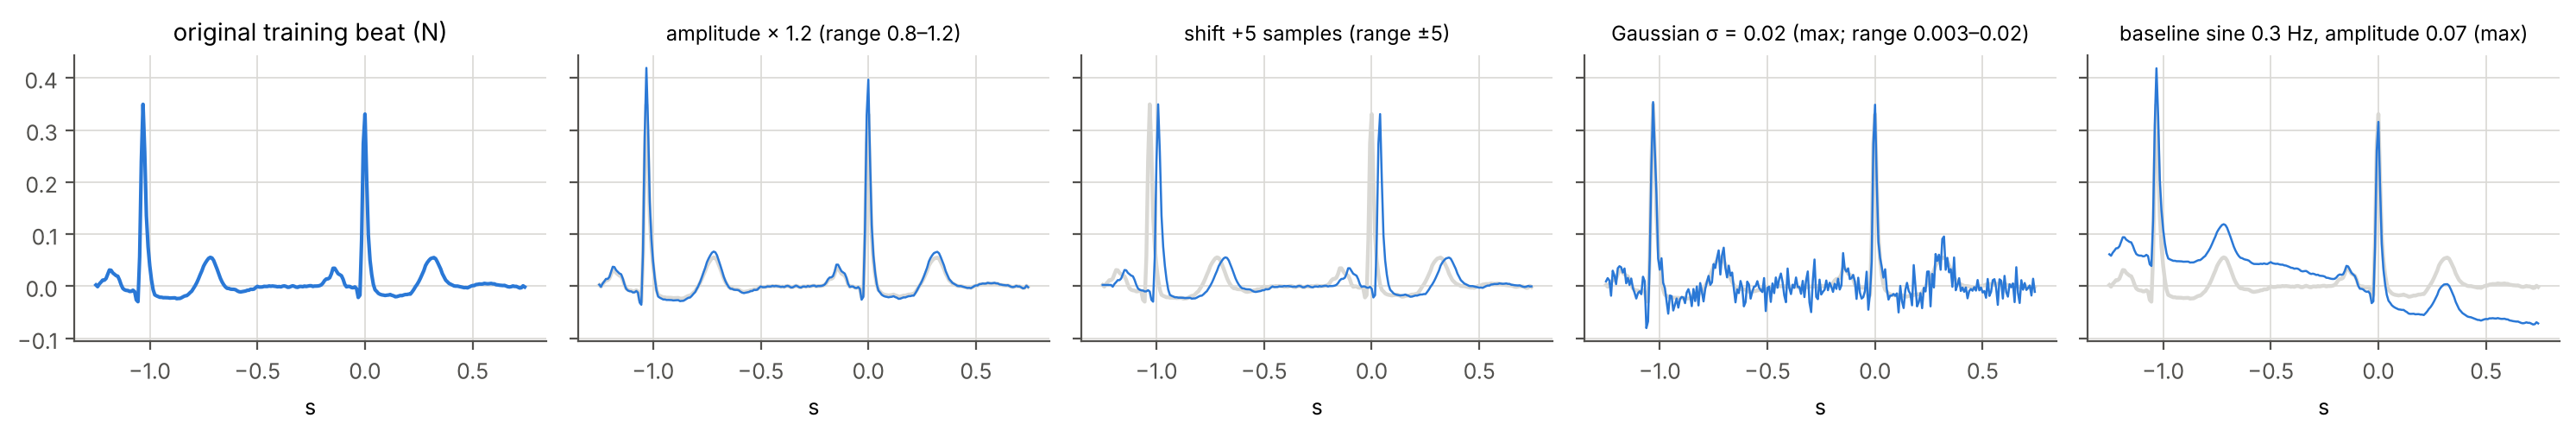
\includegraphics[width=\textwidth]{fig_augmentation.png}
\caption{Each augmentation at its strongest setting (grey: original beat).}
\label{fig:aug}
\end{figure}

\subsection{Final Dataset}

\begin{table}[H]
\centering
\small
\caption{Final dataset (\code{results/split\_stats.csv}). The 44 records come from 43 people, because validation record 201 and test record 202 are the same person.}
\label{tab:final}
\begin{tabular}{@{} l c r r r r r @{}}
\toprule
Split & Subjects/records & N & S & V & F & Total \\
\midrule
Train (DS1) & 17 / 17 & 36,489 & 615 & 3,052 & 393 & 40,549 \\
Validation (DS1) & 5 / 5 & 9,323 & 328 & 734 & 21 & 10,406 \\
Test (DS2) & 22 / 22 & 44,208 & 1,837 & 3,219 & 388 & 49,652 \\
\midrule
Total & 43 / 44 & 90,020 & 2,780 & 7,005 & 802 & 100,607 \\
\bottomrule
\end{tabular}
\end{table}

As a check, our counts are very close to those published by \citet{dechazal2004automatic} (DS1: 45,866 / 944 / 3,788 / 415 for N / S / V / F). No class differs by more than 54 beats; the difference is the beats we drop at the start and end of records.

\subsection{Reproducibility}

\begin{table}[H]
\centering
\small
\caption{Settings needed to reproduce the data (\code{configs/data.yaml}, \code{results/environment\_prepare.json}).}
\label{tab:repro}
\begin{tabularx}{\textwidth}{@{} l L @{}}
\toprule
Item & Value \\
\midrule
Software & Python 3.13.16; NumPy 2.5.3, SciPy 1.18.1, pandas 3.0.5, wfdb 4.3.1~\citep{wfdb_python}, Matplotlib 3.11.2, scikit-learn 1.9.1, PyYAML 6.0.3, PyTorch 2.14.1 (all pinned in \code{requirements.txt}); ai8x tools with their own Python 3.11 / PyTorch 2.3.1 environment (Section~\ref{sec:toolchain}) \\
Data & PhysioNet \code{mitdb} 1.0.0 and \code{nstdb} 1.0.0 \\
Random seed & 42 (training, leakage test split), 123 (noise positions). Preprocessing has no random steps. \\
Sampling frequency & 360~Hz raw, 128~Hz model input \\
Preprocessing & Band-pass 0.5--40~Hz (order 2); window 450 + 270 samples; resample to 256; subtract median; divide by $3 \times$ record beat peak; clip to $[-1, 127/128]$ \\
Input size & $2 \times 256$ (ECG and RR ratio) \\
How to run & \code{python src/prepare\_data.py -{}-config configs/data.yaml -{}-download}, then \code{notebooks/EDA.ipynb} (about one minute each); the training and evaluation commands are listed in the README \\
\bottomrule
\end{tabularx}
\end{table}

Running the preparation again gives exactly the same files and numbers. The README explains how to download the data and run each step.

% =====================================================================
\part*{Task 2: Modeling, Evaluation and Deployment}
\addcontentsline{toc}{part}{Task 2: Modeling, Evaluation and Deployment}

\section{Modeling}
% =====================================================================

Everything in Sections 4 to 6 was trained and selected on the DS1 records only. The DS2 test records were used once, for the numbers in Section~\ref{sec:evaluation}.

\subsection{Baseline}

The baseline is a random forest (200 trees, balanced class weights) on simple features: every 4th sample of the ECG window (64 values) and the RR ratio. It needs no tuning and shows what a classic method reaches on the same data. On the validation records it gets a macro F1 of 0.395; on DS2 it gets 0.475 (Table~\ref{tab:clean}). It finds almost no S beats (recall 0.04) and no F beats at all: with these simple features the rare classes are hidden behind the N class.

\subsection{Proposed Edge Model}
\label{sec:model}

The edge model is a small 1D CNN (\code{src/model.py}). It uses only layers the MAX78002 accelerator supports: 1D convolutions with kernel 3 or 5 and stride 1, max-pooling, ReLU, and one small fully connected layer. There is no batch normalisation, so the trained network is exactly what the device runs.

\begin{table}[H]
\centering
\small
\caption{Layers of the edge model (input $2 \times 256$, output 4 class scores).}
\label{tab:arch}
\begin{tabular}{@{} l l l l r @{}}
\toprule
Layer & Input & Operation & Output & Parameters \\
\midrule
conv1 & $2 \times 256$ & Conv1d k5, ReLU & $16 \times 256$ & 176 \\
conv2 & $16 \times 256$ & MaxPool 2, Conv1d k5, ReLU & $32 \times 128$ & 2,592 \\
conv3 & $32 \times 128$ & MaxPool 4, Conv1d k3, ReLU & $32 \times 32$ & 3,104 \\
conv4 & $32 \times 32$ & MaxPool 4, Conv1d k3, ReLU & $32 \times 8$ & 3,104 \\
fc & 256 (flattened) & Linear & 4 & 1,028 \\
\midrule
Total & & & & 10,004 \\
\bottomrule
\end{tabular}
\end{table}

\textbf{Why it suits Edge-AI.} It has 10,004 parameters (10~KB as INT8, 0.4\,\% of the MAX78002 weight memory) and needs 492,544 multiply--accumulate operations per beat. The pooling steps shrink the signal so that the last layers see the whole 2~s window, including the previous beat. The RR ratio enters as a second input channel, so no extra layer type is needed. We also tried a larger version with six convolution layers and 43,956 parameters; it was not better (Section~\ref{sec:selection}).

\subsection{Training Configuration}

\begin{table}[H]
\centering
\small
\caption{Training settings (\code{configs/train.yaml}).}
\label{tab:trainconf}
\begin{tabularx}{\textwidth}{@{} l L @{}}
\toprule
Setting & Value \\
\midrule
Optimiser & Adam, learning rate 0.001, weight decay 0.0001, cosine learning-rate schedule \\
Batch size / epochs & 256 / up to 40 \\
Loss function & Cross-entropy with class weights $(n_{\max}/n_c)^{0.5}$ scaled to a mean of 1: N 0.18, S 1.41, V 0.63, F 1.77 \\
Early stopping & Keep the epoch with the best validation macro F1; stop after 10 epochs without improvement (best epoch 15, stopped at 25) \\
Augmentation & Training beats only: amplitude 0.8--1.2, shift $\pm 5$ samples, Gaussian noise, baseline wander (Section~\ref{sec:aug}) \\
Random seed & 42 \\
Hardware & 2-core CPU, no GPU; one training run takes about 4 minutes \\
\bottomrule
\end{tabularx}
\end{table}

\subsection{Model Selection}
\label{sec:selection}

We trained six versions and compared them on the validation records (Table~\ref{tab:selection}). The selection rule from Section~\ref{sec:imbalance} is macro F1, with S and V recall as tie-breakers. Focal loss has a slightly higher macro F1 (0.532 against 0.529) but finds only 13\,\% of the S beats against 34\,\%, so we keep the weighted cross-entropy model. We varied the loss, the model size, the augmentation and the RR channel; the learning rate, weight decay and kernel sizes were kept fixed. The other variants confirm the Task 1 choices: without class weights, without augmentation or without the RR channel the macro F1 falls by 0.03 to 0.05, and the larger model is no better than the small one.

\begin{table}[H]
\centering
\small
\caption{Model selection on the DS1 validation records (\code{results/model\_selection.csv}).}
\label{tab:selection}
\begin{tabular}{@{} l l r r r r r @{}}
\toprule
Run & Change from the final model & Parameters & Macro F1 & Accuracy & S recall & V recall \\
\midrule
\textbf{edge\_cnn} & none (weighted cross-entropy) & 10,004 & \textbf{0.529} & 0.924 & 0.34 & 0.69 \\
focal & focal loss ($\gamma = 2$) & 10,004 & 0.532 & 0.938 & 0.13 & 0.68 \\
large & six convolution layers & 43,956 & 0.510 & 0.945 & 0.13 & 0.68 \\
no\_weights & plain cross-entropy & 10,004 & 0.499 & 0.931 & 0.14 & 0.66 \\
no\_rr & RR channel set to zero & 10,004 & 0.493 & 0.937 & 0.17 & 0.67 \\
no\_augment & no augmentation & 10,004 & 0.480 & 0.913 & 0.24 & 0.66 \\
\bottomrule
\end{tabular}
\end{table}

\subsection{Quantization}
\label{sec:quant}

The MAX78002 computes with 8-bit integers, so the FP32 model must be quantised. We compared three versions:

\begin{itemize}
  \item \textbf{INT16 and INT8 after training} (\code{src/quantize.py}): the weights, biases and activations of the trained FP32 model are rounded to 16 or 8 bits with a power-of-two step, as on the device. The activation range of each layer is measured on 4,096 training beats. No retraining.
  \item \textbf{INT8 with quantisation-aware training (QAT)}, the version that goes to the device: the same architecture is trained in ai8x-training for 40 epochs, with the same class weights and augmentation (the learning rate is halved at epochs 15, 25 and 35 instead of the cosine schedule). From epoch 20 the weights are kept in 8-bit form during training, so the network learns to work with the rounding. The result is quantised with ai8x-synthesis and evaluated with the device's integer arithmetic simulated in PyTorch (\code{train.py -{}-evaluate -8}).
\end{itemize}

QAT is needed because rounding after training cannot be undone: if a layer loses precision the network has no chance to adapt. With QAT the network adapts during training. Table~\ref{tab:quant} shows the result on DS2. Rounding the FP32 model to INT16 changes nothing, and rounding to INT8 costs only 0.002 macro F1, so this model is already well suited to 8 bits. The QAT model reaches a higher macro F1 (0.664); it is a separate training run of 40 epochs, which ends at a different point than the FP32 run (best epoch 15), so the difference comes mainly from the training run, not from the quantisation itself. Since the QAT model is the one the device runs, it is the \emph{quantized model} in the rest of the report.

\begin{table}[H]
\centering
\small
\caption{FP32 against quantised models on the DS2 test records (\code{results/quantization.csv}, \code{results/metrics.csv}).}
\label{tab:quant}
\begin{tabular}{@{} l r r r r r r @{}}
\toprule
Model & Weight size & Accuracy & Macro F1 & S F1 & V F1 & F F1 \\
\midrule
FP32 & 40,016 B & 0.914 & 0.611 & 0.458 & 0.807 & 0.220 \\
INT16, rounded after training & 20,008 B & 0.914 & 0.611 & 0.458 & 0.807 & 0.220 \\
INT8, rounded after training & 10,004 B & 0.913 & 0.609 & 0.449 & 0.802 & 0.225 \\
INT8, quantisation-aware training & 10,004 B & 0.932 & 0.664 & 0.527 & 0.892 & 0.271 \\
\bottomrule
\end{tabular}
\end{table}

% =====================================================================
\section{Evaluation}
\label{sec:evaluation}
% =====================================================================

All numbers in this section are from one run on the 22 DS2 test records (49,652 beats from 22 unseen patients).

\subsection{Clean Test Results}

\begin{table}[H]
\centering
\small
\caption{Results on the clean DS2 test records.}
\label{tab:clean}
\begin{tabular}{@{} l r r r @{}}
\toprule
Metric & Baseline (random forest) & FP32 edge model & Quantized model (INT8, QAT) \\
\midrule
Accuracy & 0.939 & 0.914 & 0.932 \\
Macro F1 & 0.475 & 0.611 & 0.664 \\
Model parameters & 204,356 tree nodes & 10,004 & 10,004 \\
\bottomrule
\end{tabular}
\end{table}

The baseline has the highest accuracy and the lowest macro F1: it predicts N for 99\,\% of the N beats but misses almost all S and F beats. Accuracy alone would have ranked the models the wrong way round.

\begin{figure}[H]
\centering
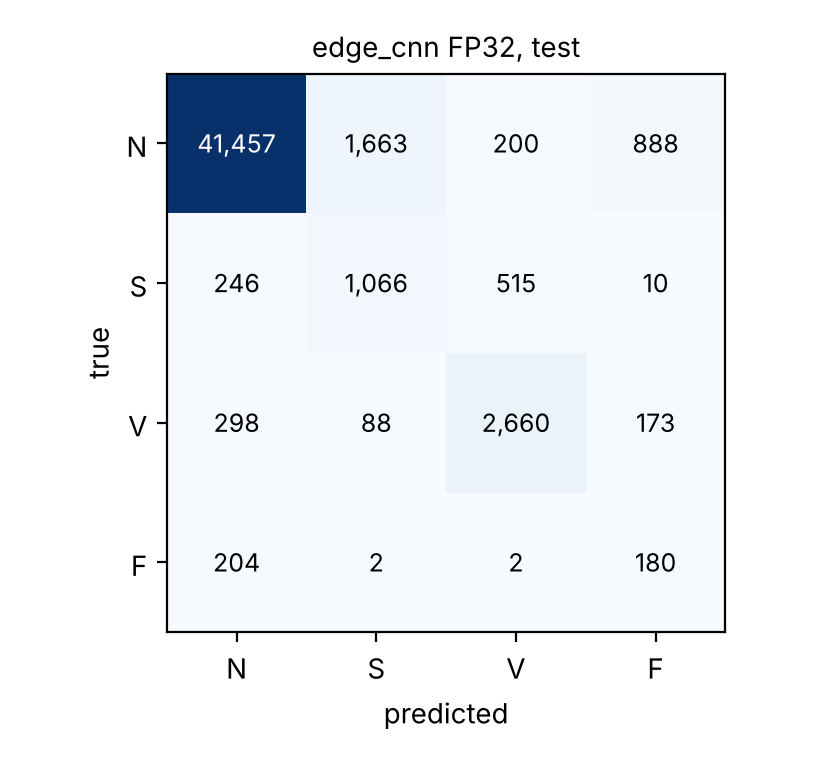
\includegraphics[width=0.42\textwidth]{task2/confusion_matrix_edge_cnn_FP32_test.png}\hfill
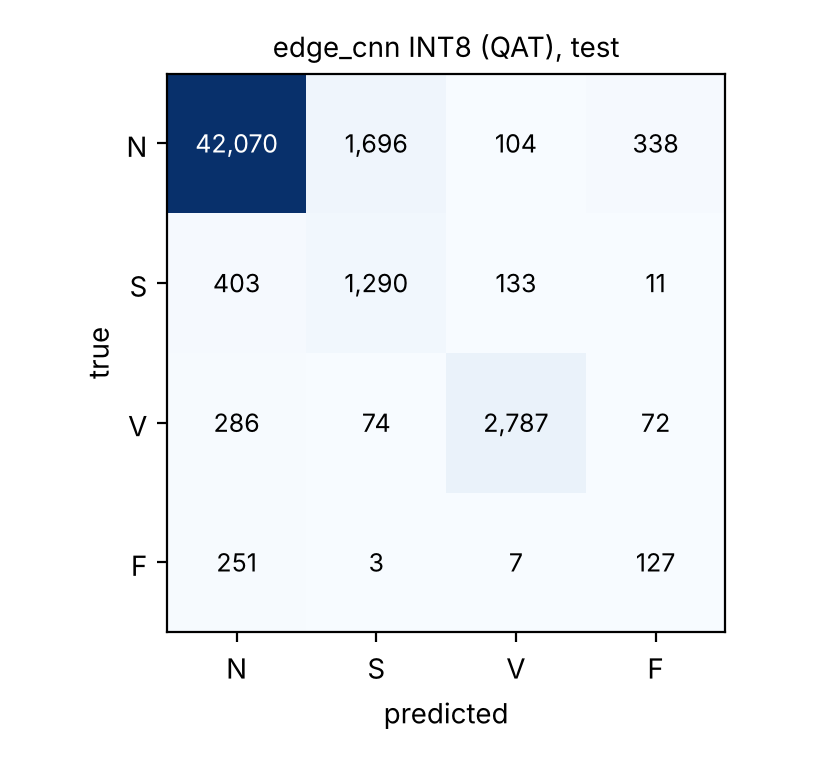
\includegraphics[width=0.42\textwidth]{task2/confusion_matrix_edge_cnn_INT8-QAT_test.png}
\caption{Confusion matrices on DS2 for the FP32 model (left) and the INT8 QAT model (right).}
\label{fig:cm}
\end{figure}

\subsection{Per-Class Performance}

\begin{table}[H]
\centering
\small
\caption{Per-class results on DS2 (FP32 model / INT8 QAT model).}
\label{tab:perclass}
\begin{tabular}{@{} l r r r r @{}}
\toprule
Class & Beats & Precision & Sensitivity / recall & F1 \\
\midrule
N & 44,208 & 0.982 / 0.978 & 0.938 / 0.952 & 0.960 / 0.965 \\
S & 1,837 & 0.378 / 0.421 & 0.580 / 0.702 & 0.458 / 0.527 \\
V & 3,219 & 0.788 / 0.920 & 0.826 / 0.866 & 0.807 / 0.892 \\
F & 388 & 0.144 / 0.232 & 0.464 / 0.327 & 0.220 / 0.271 \\
\bottomrule
\end{tabular}
\end{table}

\textbf{Which classes are difficult and why.} V is the easiest rare class: its wide shape is visible in every patient. S is hard because an S beat looks like an N beat and only its timing differs; the model finds 58--70\,\% of them, but more than half of the ``S'' predictions are in fact early N beats, which keeps S precision low. F is the hardest: there are only 388 F beats, 93\,\% of them from one patient (record 213), and in training F came almost entirely from another single patient (record 208). The model learned one patient's fusion shape, which transfers poorly.

\subsection{Quantization Analysis}

FP32 macro F1: \textbf{0.611}. INT8 macro F1: \textbf{0.609} after plain rounding, \textbf{0.664} with quantisation-aware training. Difference: $-0.002$ for plain rounding, within the $-0.02$ limit of criterion Q2; INT16 rounding changes nothing (criterion Q3). Quantisation costs this model very little: the inputs were already prepared for the 8-bit range in Task 1, the network is small, and all weights are small (the largest magnitude is 0.91 in the first layer and 0.42--0.66 in the others), so no layer needs a coarse step. The class that moves most under plain INT8 rounding is S (F1 $-0.009$), the class with the smallest margins.

\subsection{Noise Robustness}

Real noise from the Noise Stress Test Database was added to the raw DS2 signals (Section~\ref{sec:eda}), the beats were prepared with the identical pipeline, and the frozen FP32 model and its INT8 version were evaluated (\code{src/noise\_test.py}). Table~\ref{tab:noise} gives the mixed noise; Figure~\ref{fig:noise_results} shows each noise type.

\begin{table}[H]
\centering
\small
\caption{Results under mixed noise (bw + ma + em), FP32 model (\code{results/noise\_results.csv}).}
\label{tab:noise}
\begin{tabular}{@{} l r r r r r r @{}}
\toprule
Condition & Accuracy & Macro F1 & N recall & S recall & V recall & F recall \\
\midrule
Clean & 0.914 & 0.611 & 0.938 & 0.580 & 0.826 & 0.464 \\
12 dB & 0.885 & 0.563 & 0.908 & 0.519 & 0.830 & 0.474 \\
6 dB & 0.814 & 0.479 & 0.831 & 0.452 & 0.842 & 0.420 \\
0 dB & 0.658 & 0.349 & 0.664 & 0.341 & 0.815 & 0.266 \\
\bottomrule
\end{tabular}
\end{table}

\begin{figure}[H]
\centering
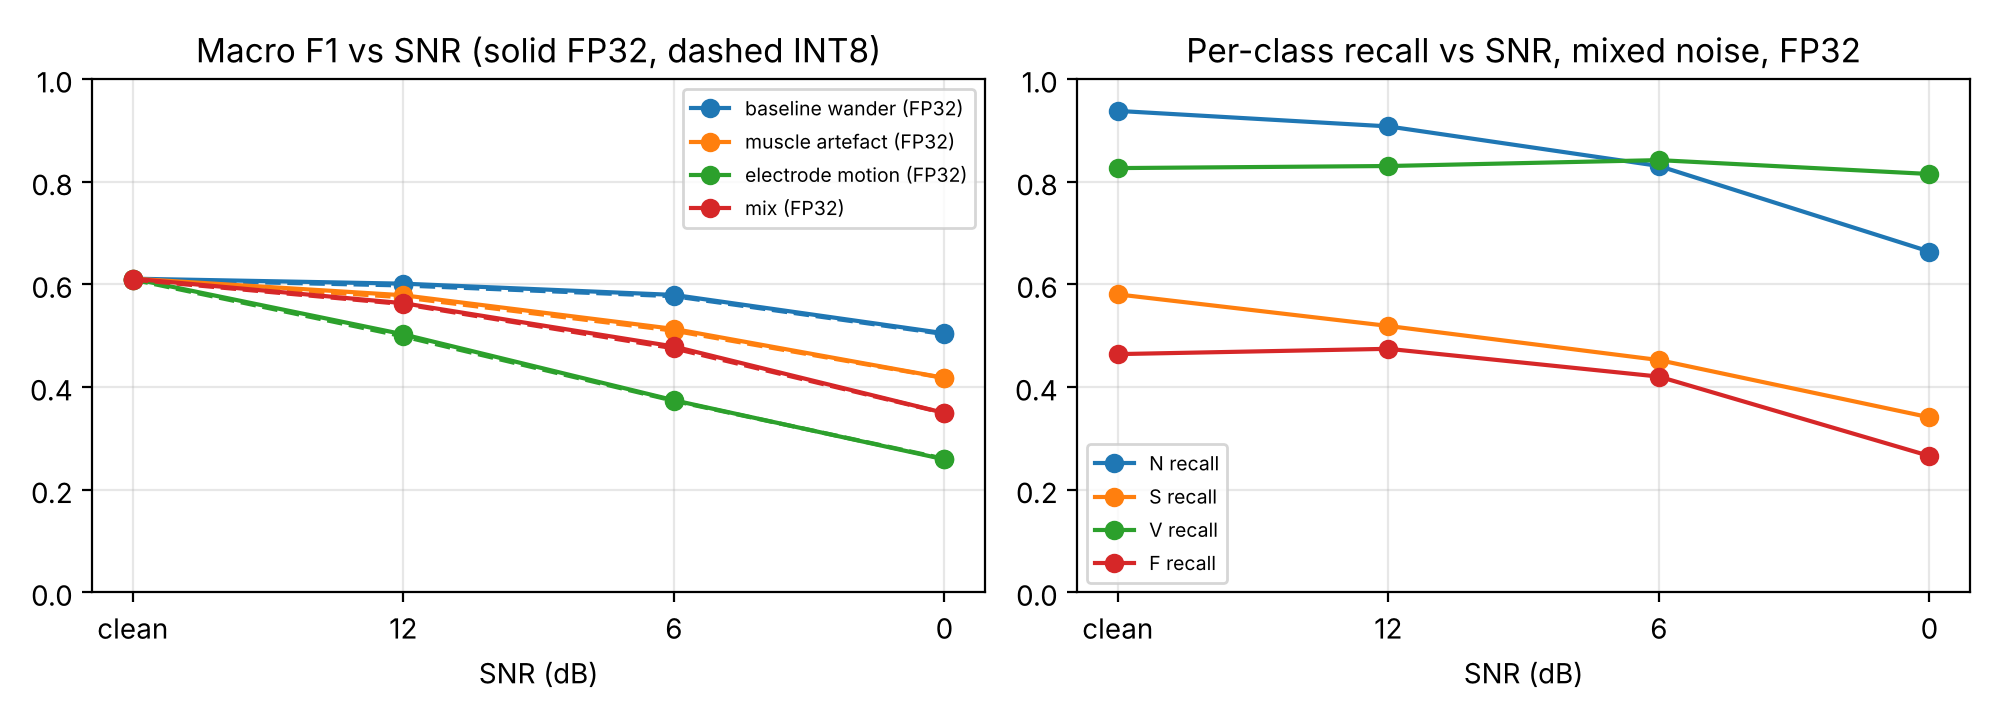
\includegraphics[width=\textwidth]{task2/noise_results.png}
\caption{Left: macro F1 against SNR for each noise type (FP32 solid, INT8 dashed; the two lines overlap). Right: per-class recall under mixed noise.}
\label{fig:noise_results}
\end{figure}

\begin{itemize}
  \item \textbf{Most affected classes:} N and S. Under noise the model calls more and more N beats S or V (N recall falls from 0.94 to 0.66 at 0~dB), and S recall falls to 0.34. V recall stays above 0.77 for every noise type and level: wide V beats are visible even through strong noise.
  \item \textbf{Degradation is gradual} for baseline wander and muscle noise (macro F1 0.60 and 0.58 at 12~dB) and much steeper for electrode motion (0.50 at 12~dB, 0.26 at 0~dB). Averaged over the three noise types the macro F1 drops by 0.050 at 12~dB, 0.122 at 6~dB and 0.217 at 0~dB.
  \item \textbf{Preprocessing helps} against baseline wander, which the 0.5~Hz high-pass filter removes for the most part (macro F1 costs 0.01 at 12~dB and 0.03 at 6~dB, but 0.11 at 0~dB). It cannot help against electrode motion, whose spikes lie inside the 0.5--40~Hz band and look like beats (Figure~\ref{fig:noise_errors}).
  \item \textbf{Robustness could be improved} by training with real noise from the reserved first half of the noise records, by a signal-quality check that rejects beats like the one in the lower right of Figure~\ref{fig:noise_errors}, and by a longer window that averages over more beats. INT8 does not change robustness: the INT8 curves lie on top of the FP32 curves.
\end{itemize}

\subsection{Error Analysis}

Figures~\ref{fig:err_ns}--\ref{fig:noise_errors} show representative misclassified beats of the FP32 model (all examples in \code{results/errors/}).

\textbf{N classified as S (1,663 beats).} About two thirds (1,142) come from records 222, 219 and 221, which contain atrial fibrillation and flutter. In these rhythms normal beats arrive at irregular times, and the median RR ratio of the misclassified beats is 0.80, against 1.01 for correct N beats. The model has learned ``early beat with normal shape = S'', which is right for a regular rhythm but wrong in fibrillation.

\begin{figure}[H]
\centering
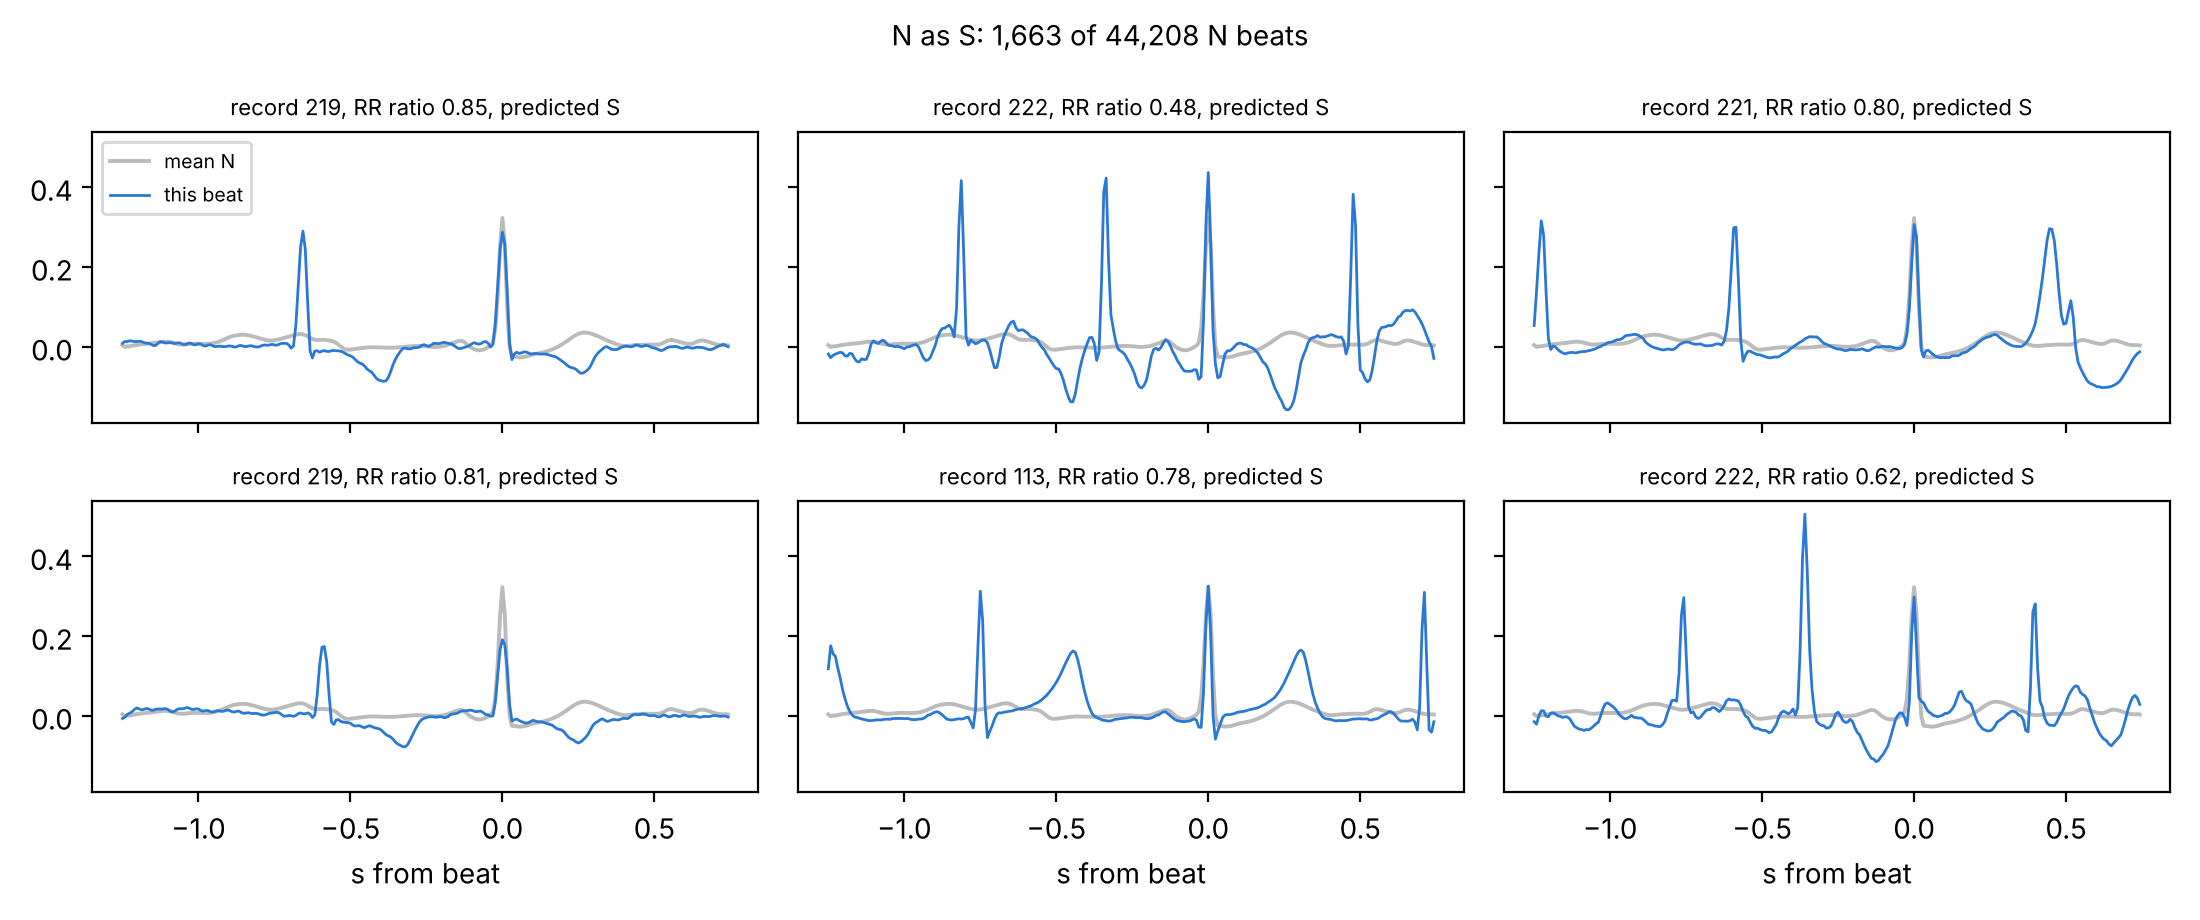
\includegraphics[width=\textwidth]{task2/N_as_S.png}
\caption{N beats classified as S: normal shape, but the beat came early because the rhythm is irregular.}
\label{fig:err_ns}
\end{figure}

\textbf{S classified as N (246 beats) or V (515 beats).} Almost all come from record 232 (168 of the S$\to$N and 447 of the S$\to$V errors). This patient has a slow rhythm with long pauses. The S beats called N have RR ratios of 0.9--1.0, so they do not look early and the model falls back on the shape, which is normal (Figure~\ref{fig:err_sn}). The S beats called V do arrive early (median RR ratio 0.67), but their shape, with the patient's unusual T-wave, is taken for a wide V beat.

\begin{figure}[H]
\centering
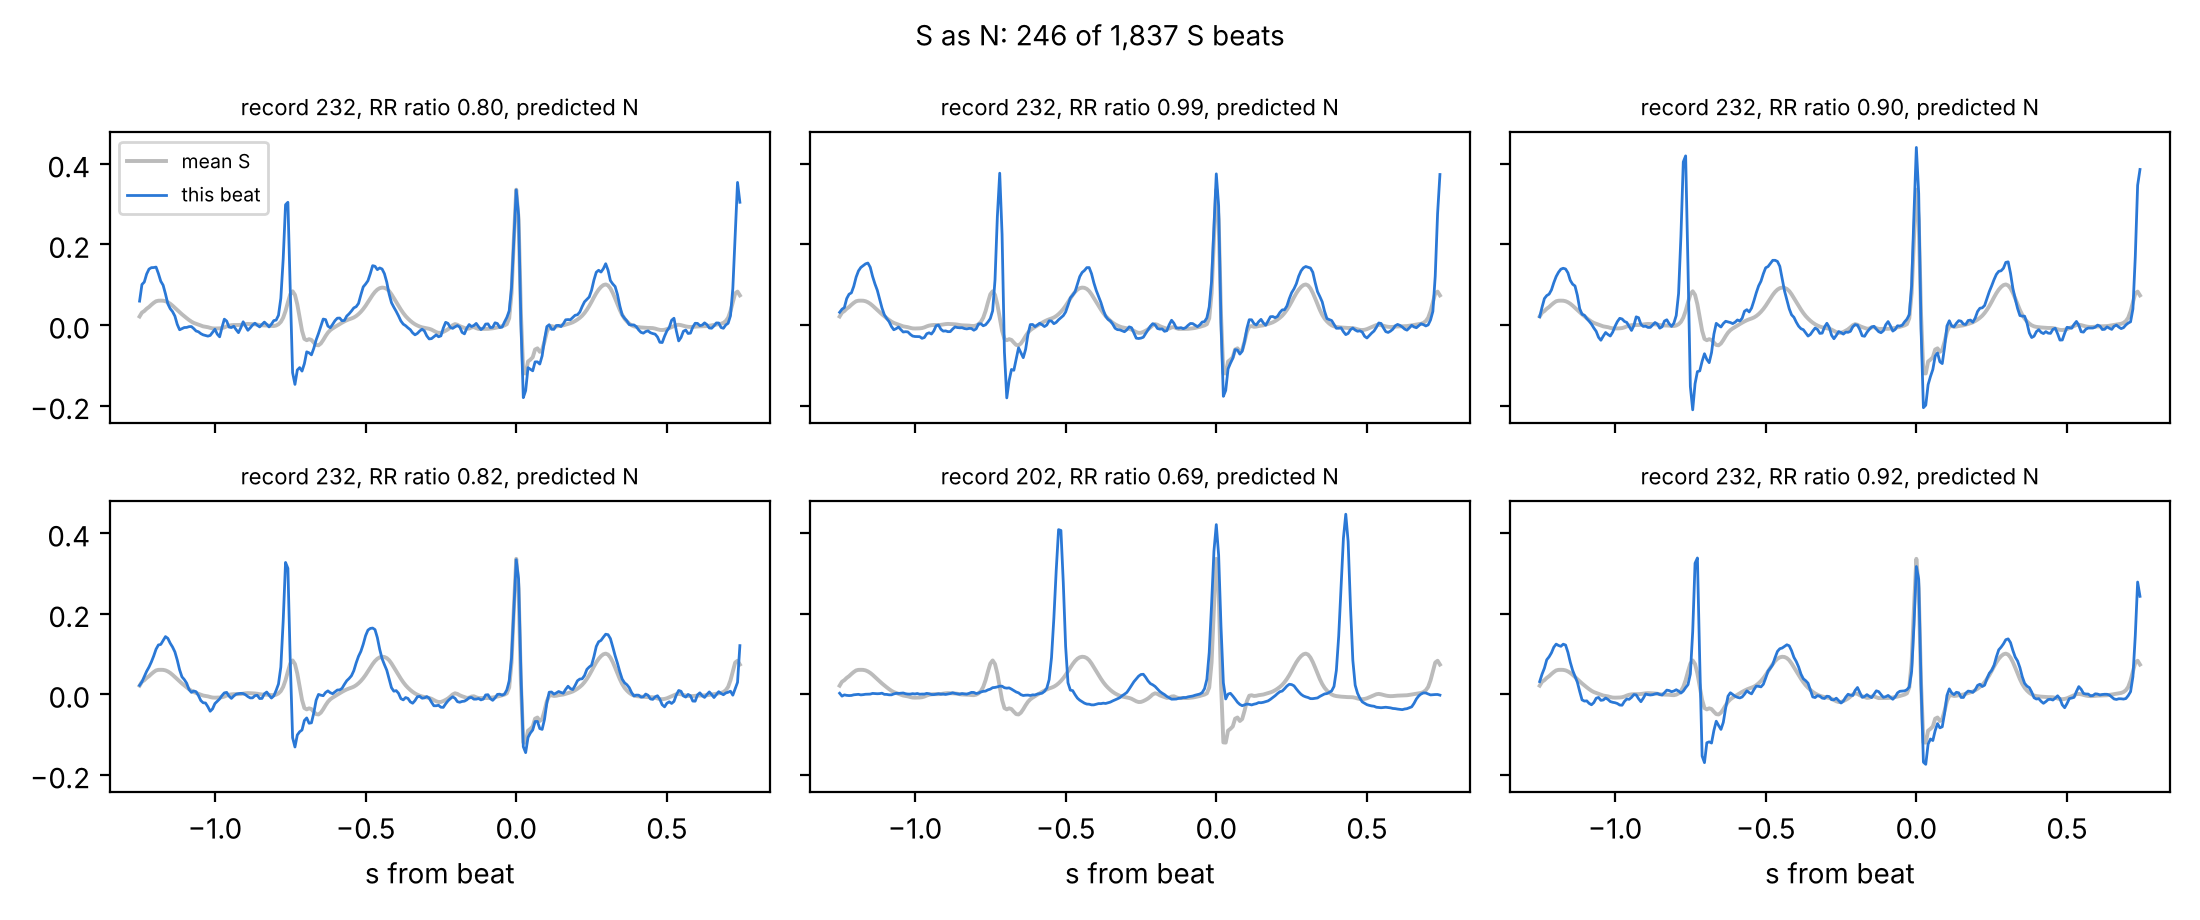
\includegraphics[width=\textwidth]{task2/S_as_N.png}
\caption{S beats classified as N, mostly from record 232: normal shape and an RR ratio close to 1.}
\label{fig:err_sn}
\end{figure}

\textbf{V classified incorrectly (559 beats).} 298 were called N, 196 of them in record 233, whose V beats are narrower than the training V beats (Figure~\ref{fig:err_v}). Another 173 were called F, which is the neighbouring class by definition.

\begin{figure}[H]
\centering
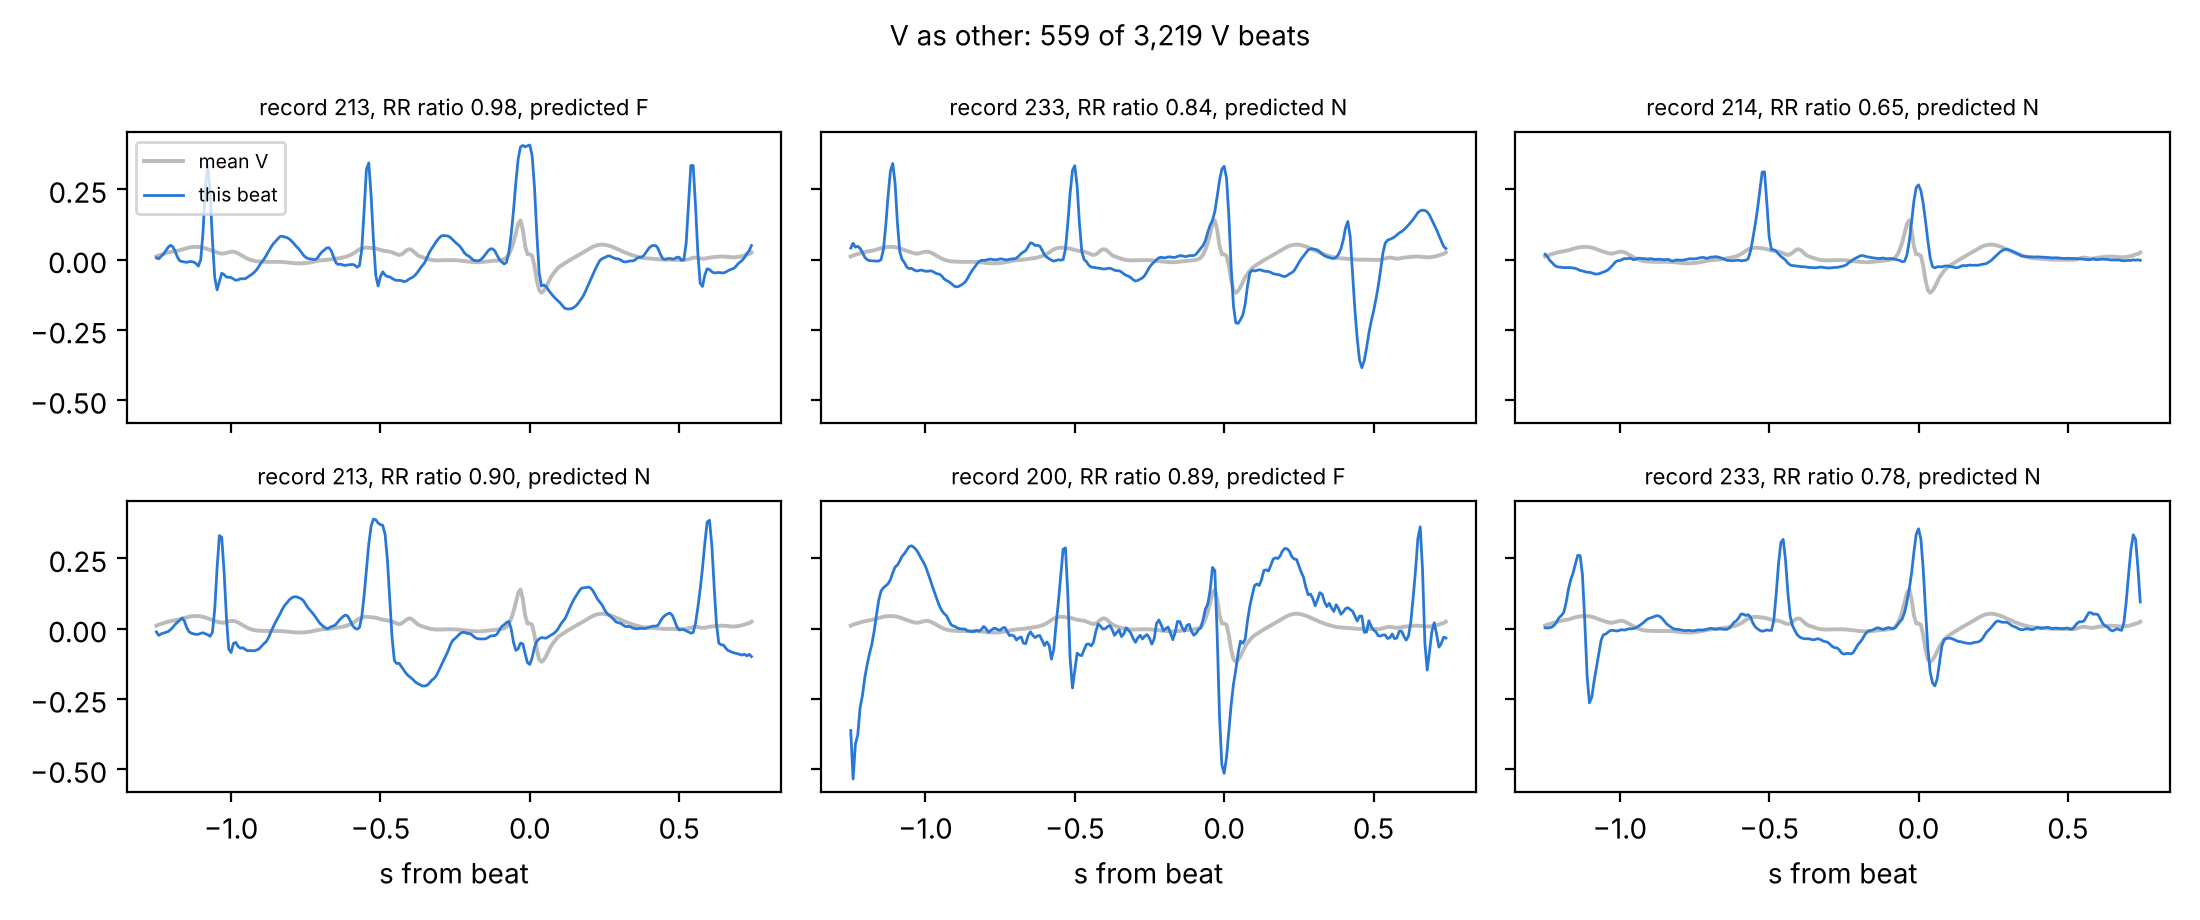
\includegraphics[width=\textwidth]{task2/V_as_other.png}
\caption{V beats classified as N or F: narrower than the average V beat.}
\label{fig:err_v}
\end{figure}

\textbf{F classified incorrectly (208 beats).} 204 were called N, 185 of them in record 213. Figure~\ref{fig:err_f} shows why: these fusion beats differ from a normal beat only by a slightly wider QRS, at normal timing.

\begin{figure}[H]
\centering
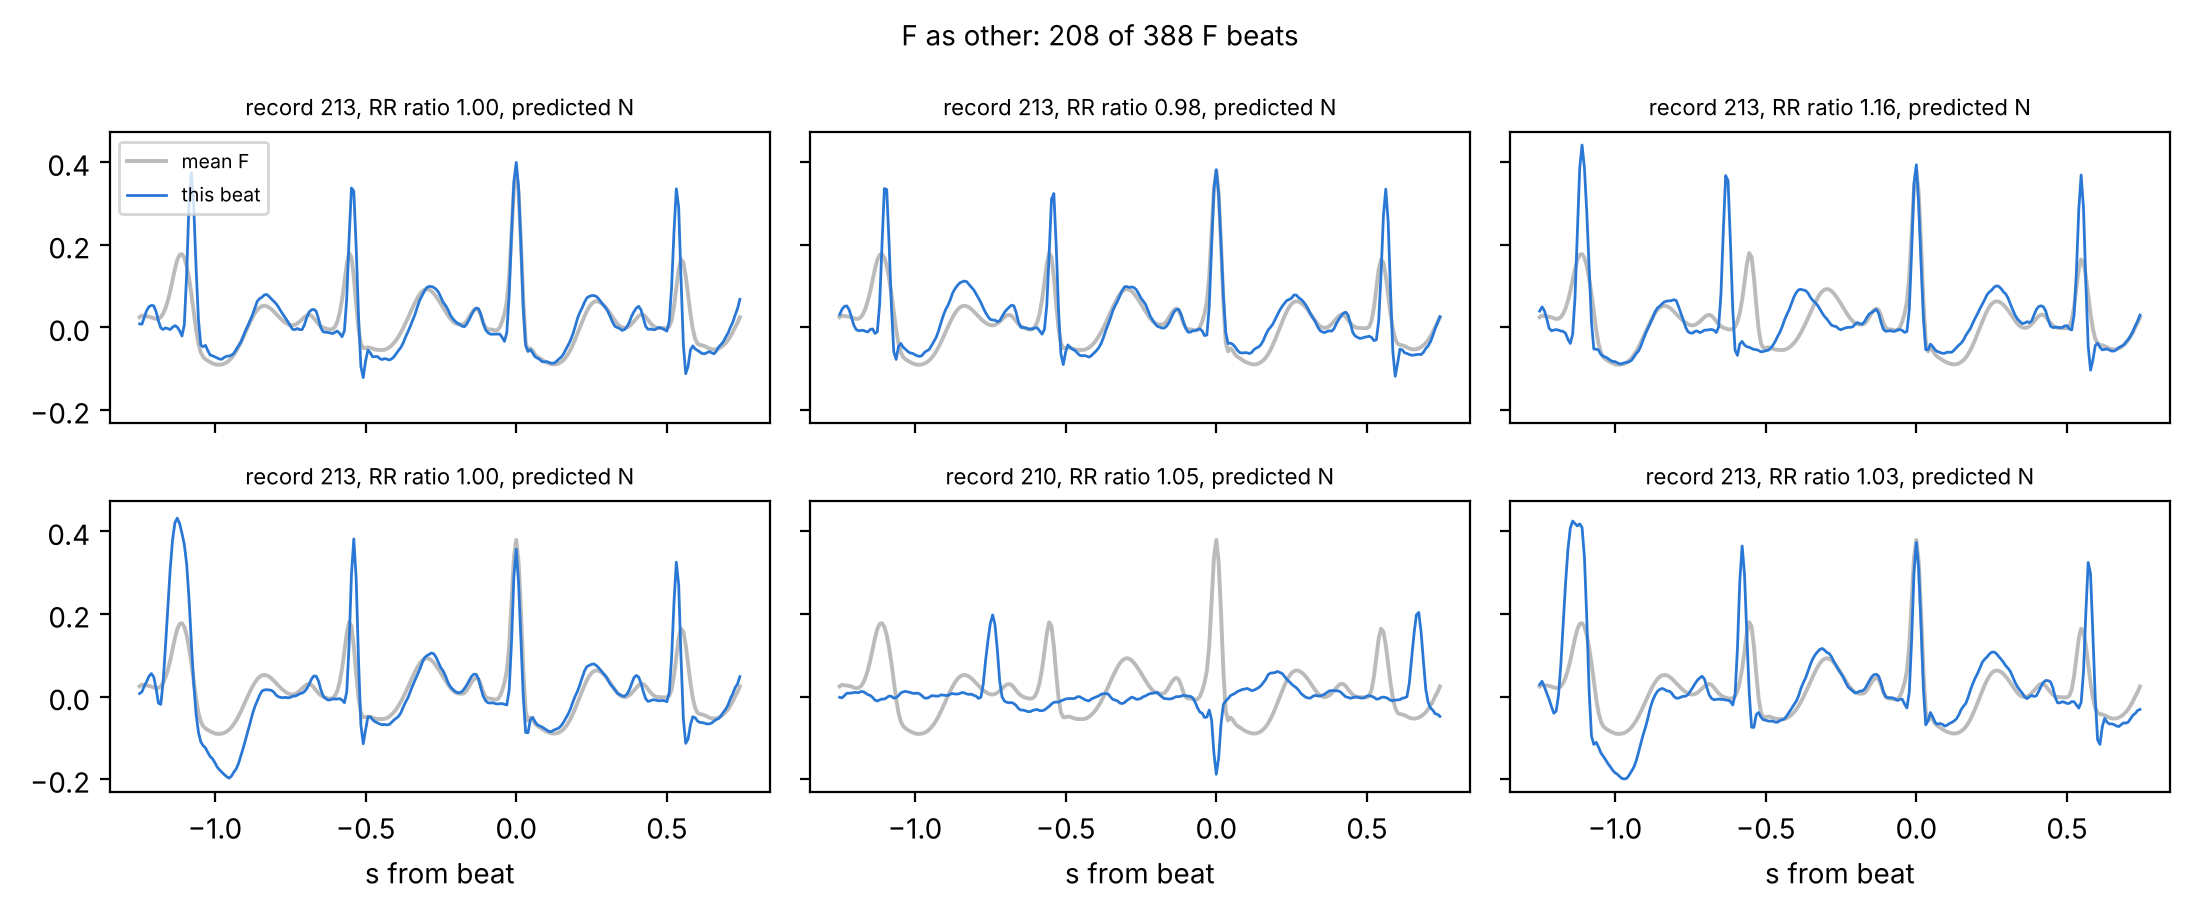
\includegraphics[width=\textwidth]{task2/F_as_other.png}
\caption{F beats classified as N: the shape is close to normal and the timing is regular.}
\label{fig:err_f}
\end{figure}

\textbf{Errors under strong noise.} At 0~dB mixed noise, 1,027 S, V and F beats that were correct when clean become wrong. Figure~\ref{fig:noise_errors} shows that electrode-motion spikes near the beat change the apparent width of the QRS complex, so S and F beats are called V, and that large baseline swings push the signal to the clipping limit.

\begin{figure}[H]
\centering
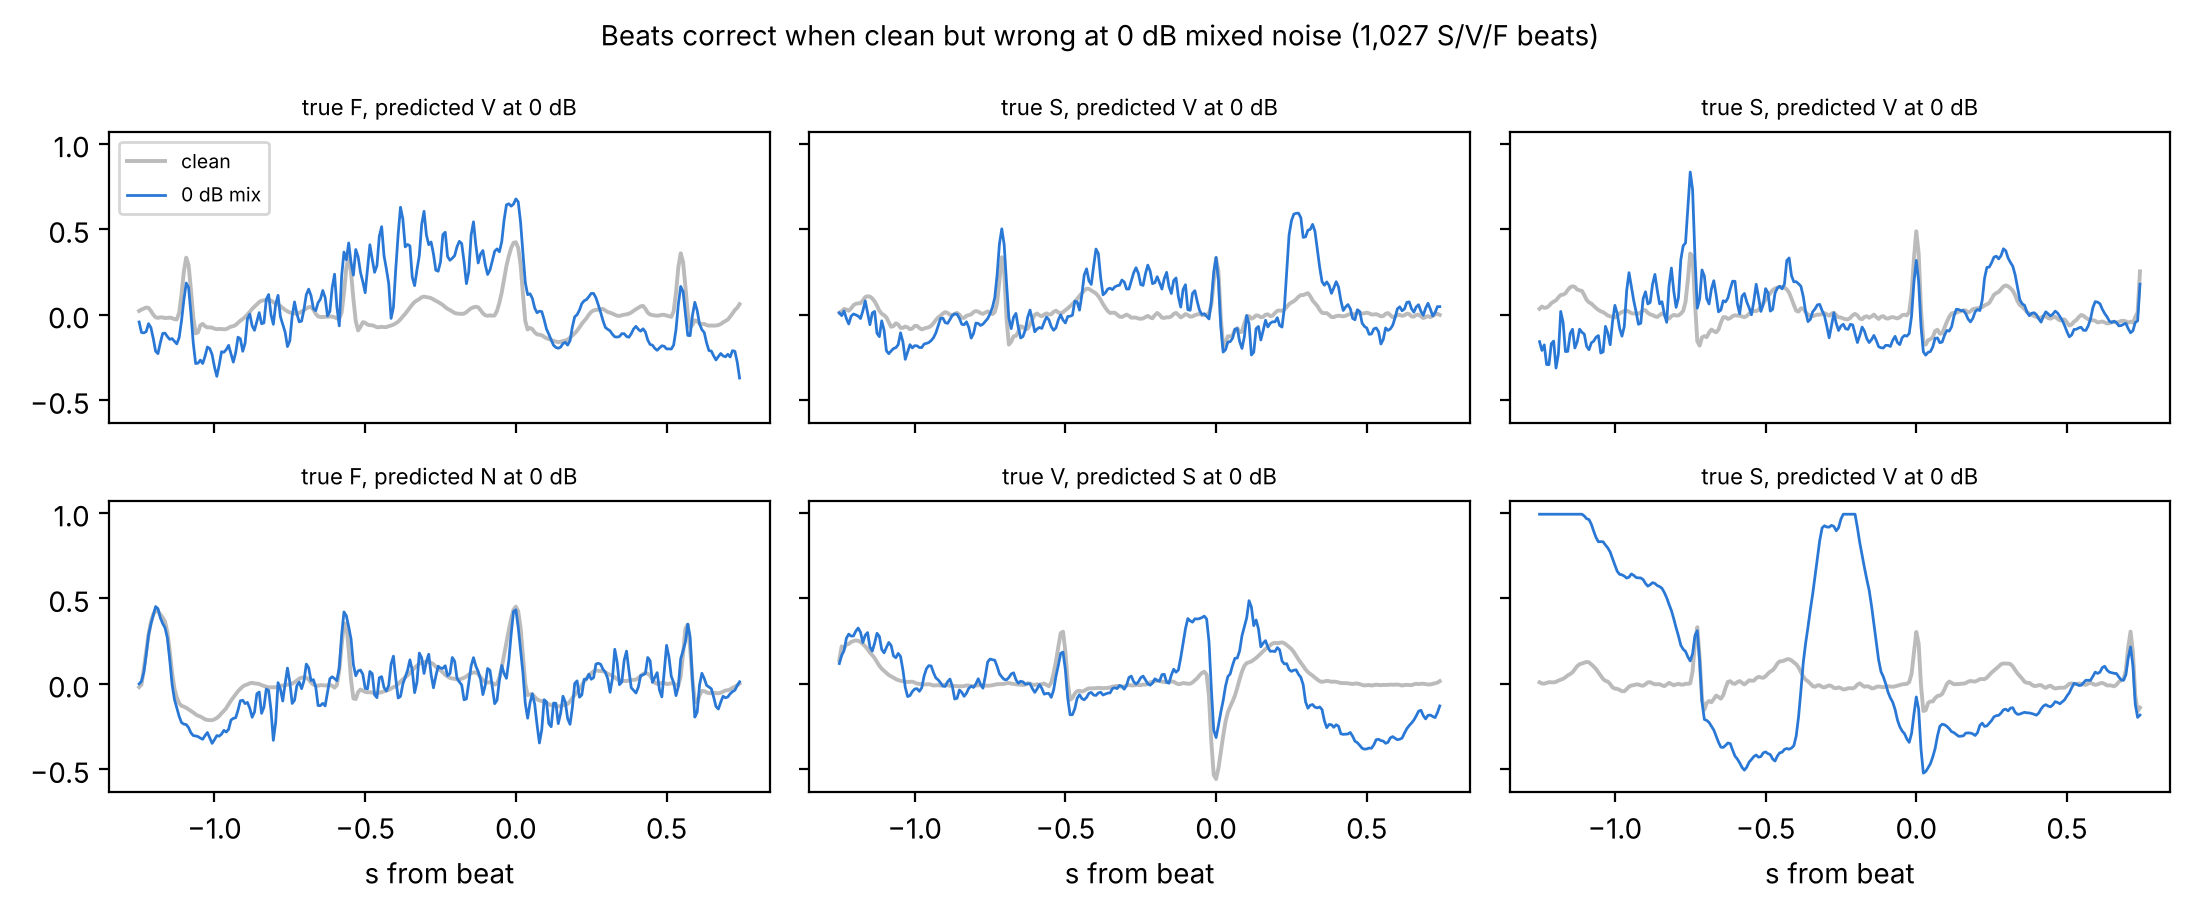
\includegraphics[width=\textwidth]{task2/noise_0dB.png}
\caption{Beats correct when clean (grey) but wrong at 0~dB mixed noise (blue).}
\label{fig:noise_errors}
\end{figure}

\subsection{Success-Criteria Review}

Table~\ref{tab:review} returns to the criteria of Table~\ref{tab:success}. The status is judged on the quantized model (the one the device runs) where the criterion does not name a model; FP32 values are given for comparison.

\begin{table}[H]
\centering
\small
\caption{Review of the success criteria on DS2.}
\label{tab:review}
\begin{tabularx}{\textwidth}{@{} l >{\raggedright\arraybackslash}p{5.6cm} l l L @{}}
\toprule
ID & Criterion (target) & FP32 & INT8 QAT & Status \\
\midrule
P1 & Macro F1 of the FP32 model $\geq 0.60$ & 0.611 & 0.664 & Achieved \\
P2 & Macro F1 gain over the baseline $\geq +0.05$ & $+0.136$ & $+0.188$ & Achieved (stretch) \\
P3 & N recall $\geq 0.90$ & 0.938 & 0.952 & Achieved (stretch) \\
M1 & V recall / precision $\geq 0.80$ / $0.70$ & 0.826 / 0.788 & 0.866 / 0.920 & Achieved \\
M2 & S recall / precision $\geq 0.60$ / $0.40$ & 0.580 / 0.378 & 0.702 / 0.421 & Achieved (INT8); FP32 just below \\
M3 & F recall $\geq 0.25$ & 0.464 & 0.327 & Achieved \\
R1 & Macro F1 drop at 12 dB $\leq 0.05$ (mean of bw, ma, em) & 0.0502 & -- & Partially achieved (at the limit) \\
R2 & Macro F1 drop at 6 dB $\leq 0.10$ & 0.122 & -- & Not achieved \\
R3 & V recall at 0 dB $\geq 0.50$ & 0.805 & -- & Achieved (stretch) \\
C1 & Parameters $\leq 100{,}000$ & 10,004 & 10,004 & Achieved (stretch) \\
C2 & INT8 weight memory $\leq 100$ KB & -- & 9,888 B & Achieved (stretch) \\
C3 & MACs per beat $\leq 5$ M & 0.49 M & 0.49 M & Achieved (stretch) \\
Q1 & FP32, INT16 and INT8 compared & \multicolumn{2}{l}{Table~\ref{tab:quant}} & Achieved \\
Q2 & INT8 minus FP32 macro F1 $\geq -0.02$ & \multicolumn{2}{l}{$-0.002$ (rounding), $+0.053$ (QAT)} & Achieved (stretch) \\
Q3 & INT16 minus FP32 macro F1 $\geq -0.005$ & \multicolumn{2}{l}{0.000} & Achieved (stretch) \\
H1 & Only supported layers, fixed $2 \times 256$ input & \multicolumn{2}{l}{yes} & Achieved \\
H2 & Toolchain: accepted, quantised, synthesised, C files & \multicolumn{2}{l}{4 $\times$ PASS} & Achieved \\
\bottomrule
\end{tabularx}
\end{table}

The noise test on R1--R3 used the FP32 model and its INT8-rounded copy, which give the same curves (Figure~\ref{fig:noise_results}). The one clear miss is R2: at 6~dB the model loses 0.12 macro F1, mostly because of electrode-motion noise. We set that target before seeing how strong electrode motion is at 6~dB with the proper SNR definition (Section~\ref{sec:eda}); the target was too optimistic for a model trained without real noise.

% =====================================================================
\section{Deployment}
\label{sec:toolchain}
% =====================================================================

In this course, deployment means preparing the model for the MAX78002 with the Analog Devices software. No board was used.

\subsection{MAX78002 Compatibility}

\begin{itemize}
  \item \textbf{Layer types:} Conv1d (kernels 5 and 3, stride 1, padding 2 and 1), MaxPool1d (2 and 4), ReLU, one Linear layer. All are in the accelerator's supported list; the kernel lengths are within the 1--9 limit, pooling within 1--16, and the Linear layer has 256 inputs and 4 outputs (limit 1,024)~\citep{adi_ai8x_training}.
  \item \textbf{Input:} a fixed $2 \times 256$ array of signed 8-bit values. \textbf{Output:} 4 class scores (32-bit); the softmax runs on the CPU.
  \item \textbf{Parameters:} 10,004, all 8-bit. At most 32 channels per layer, so every layer fits in one pass of the 64 processors.
\end{itemize}

\subsection{MAX78002 Toolchain}

We used ai8x-training (commit 2dfe594) and ai8x-synthesis (commit 7379b29)~\citep{adi_ai8x_training,adi_ai8x_synthesis}, each in its own Python 3.11 environment with PyTorch 2.3.1; the commits are pinned in \code{max78002/README.md}. The model is written with the ai8x layers (\code{max78002/model\_configuration/ai85ecgnet.py}), the beats are loaded with our own dataset file, and the network layout for the synthesiser is in \code{ecg\_mitbih.yaml}. The four steps, with the exact commands in \code{max78002/README.md}:

\begin{enumerate}
  \item \textbf{Train with QAT} (\code{train.py}, 40 epochs, 8-bit weights from epoch 20, record-level validation kept with \code{-{}-validation-split 0}).
  \item \textbf{Quantise} the checkpoint with \code{quantize.py}.
  \item \textbf{Evaluate in 8-bit mode} (\code{train.py -{}-evaluate -8}): validation macro F1 0.516, DS2 macro F1 0.664. The same command saves one known input for the self-test of the C code.
  \item \textbf{Synthesise} with \code{ai8xize.py}, which writes the C project (\code{cnn.c}, \code{weights.h}, \code{main.c}, \code{sampledata.h}, \code{sampleoutput.h}, Makefile).
\end{enumerate}

The toolchain keeps the checkpoint with the best accuracy, which for this data favours N. We therefore used the checkpoint of the last QAT epoch, without any selection on the validation set.

\subsection{Deployment Evidence}

\begin{table}[H]
\centering
\small
\caption{Toolchain results (\code{max78002/quantization\_output/}, \code{max78002/synthesis\_output/}).}
\label{tab:deploy}
\begin{tabularx}{\textwidth}{@{} >{\raggedright\arraybackslash}p{3.6cm} L @{}}
\toprule
Requirement & Result \\
\midrule
Model accepted by MAX78002 toolchain & PASS (ai8x-training trained it; ai8xize.py accepted the checkpoint and the network description) \\
Quantization completed & PASS (quantize.py wrote 8-bit weights and biases for all 5 layers; \code{quantization\_output/quantize.log}) \\
Synthesis completed & PASS (ai8xize.py finished without errors; \code{synthesis\_output/ai8xize.log}) \\
C/device files generated & PASS (\code{synthesis\_output/ecg/}: cnn.c, cnn.h, weights.h, main.c, softmax.c, sampledata.h, sampleoutput.h, Makefile) \\
Weight-memory requirement & 9,888 bytes of 2,396,160 (0.4\,\%); bias memory 116 bytes of 8,192 \\
Data-memory requirement & largest layer output 4,096 bytes (conv1 and conv2), spread over the processors' data memory of 1,280~KiB; input 512 bytes \\
Operations per beat & 492,544 multiply--accumulate and 18,688 compare operations (from \code{main.c}) \\
\bottomrule
\end{tabularx}
\end{table}

\subsection{Hardware Limitations}
\label{sec:hwlimits}

Everything above is \emph{software verified}: the toolchain accepted the model, the INT8 accuracy comes from the bit-accurate simulation in ai8x-training, and the memory and operation counts come from the generated code. The following are \emph{not verified}, and we make no claims about them: inference latency, power consumption, energy per inference, accuracy measured on the device, and real-time behaviour.

\subsection{Proposed Hardware Validation}

If a MAX78002 evaluation kit were available, we would:
\begin{enumerate}
  \item Flash the generated project to the board. It already contains one known input (\code{sampledata.h}) and its expected output (\code{sampleoutput.h}) as a self-test.
  \item Send the DS2 beats to the board over the serial port, as the same $2 \times 256$ INT8 arrays used in Python, and read back the four scores.
  \item Compare the board's scores with the Python INT8 simulation beat by beat; they should match exactly, and any difference points to a data-format or scaling error.
  \item Read back the intermediate layer outputs for a few beats from the accelerator memory and compare them with the simulation.
  \item Measure the inference time per beat with the on-chip timer and the energy per inference with the kit's power-measurement header, and compare the time with the beat rate (about one beat per second).
\end{enumerate}

% =====================================================================
\section{Final Discussion}
% =====================================================================

\textbf{What we learned from the data.} The rare classes are rare in patients, not only in beats: F comes from one training patient and one test patient, and S from a handful. Beats of one patient are near-copies of each other, so a random split would have given a macro F1 of about 0.88 instead of the 0.61--0.66 we get on new patients. The timing of a beat (the RR ratio) matters as much as its shape.

\textbf{Largest source of error.} Rhythm, not shape. Most N$\to$S errors are normal beats that arrive early in atrial fibrillation, and most S errors are S beats that do not arrive early in a patient with a slow, irregular rhythm. These are limits of the one-beat view: the model sees 2~s, not the rhythm of the last minute.

\textbf{Was the most accurate model the best Edge-AI model?} No. The random forest has the highest accuracy (0.939) and the lowest macro F1, and it is 20 times larger than the CNN. The larger CNN had higher validation accuracy than the small one but a lower macro F1. The small CNN is the best model on macro F1 and the smallest.

\textbf{Loss after quantisation.} Very small: 0.002 macro F1 for plain INT8 rounding, 0 for INT16, and the QAT model is the best model we have.

\textbf{Sensitivity to noise.} Moderate for baseline wander and muscle noise, strong for electrode motion. V beats survive noise well; N and S do not.

\textbf{Compromises because of hardware.} Only small ones. The 8-bit input range forced the normalisation and clipping of Task 1; the supported-layer list ruled out batch normalisation and recurrent layers; and the training-time augmentation stands in for a larger model. The 2~MB memory target was never close to binding.

\textbf{With more time} we would train with real noise from the reserved half of the noise records, add a short rhythm feature over the last 10--20 beats (for example the RR variability) to separate fibrillation from premature beats, run the record-level cross-validation inside DS1 to get a more reliable validation score, and test the generated code on a MAX78002 kit.

% =====================================================================
\section{Limitations}
% =====================================================================

\begin{itemize}
  \item \textbf{Dataset size.} 44 records from 43 people. The rare classes come from very few patients: 95\,\% of the training F beats are from one record.
  \item \textbf{Class imbalance.} N is 90\,\% of the data; the S and F results rest on a few hundred beats and move by several points between training runs.
  \item \textbf{Differences between patients.} Beat shapes and rhythms differ strongly between people, and the test set contains S and V shapes the model never saw in training. The validation score (macro F1 0.53) was a poor predictor of the test score (0.61--0.66), because the five validation patients are not representative.
  \item \textbf{Historical data.} MIT-BIH was recorded in 1975--1979 on analogue tape with hospital equipment.
  \item \textbf{No clinical testing.} The model has never been tested on new patients in a clinical setting, and it is not a medical device.
  \item \textbf{No hardware testing.} All deployment results are software-level (Section~\ref{sec:hwlimits}).
  \item \textbf{Domain shift to wearables.} A wearable uses other electrodes and positions, has more motion noise, needs its own beat detector and a causal filter, and sees people moving around. Results on wearable ECG would be lower than on MIT-BIH.
\end{itemize}

% =====================================================================
\section{Final Submission Package}
% =====================================================================

{\footnotesize
\begin{verbatim}
Group15_ECG_Project/
|-- report.pdf, README.md, requirements.txt
|-- report/      LaTeX source and figures
|-- notebooks/   EDA.ipynb
|-- src/         prepare_data.py, ecg_noise.py, dataset.py, model.py, metrics.py,
|                baseline.py, train.py, evaluate.py, quantize.py, noise_test.py
|-- configs/     data.yaml, noise.yaml, train.yaml
|-- results/     metrics.csv, quantization.csv, model_selection.csv, noise_results.*,
|                confusion_matrix_*, errors/, runs/, figures/, Task 1 statistics
`-- max78002/    model_configuration/, quantization_output/, synthesis_output/, README.md
\end{verbatim}
}

The raw PhysioNet data are not included; the README explains how to download them and how to run every step in order.

\bibliographystyle{plainnat}
\bibliography{refs}

\end{document}
